\documentclass{article}


% if you need to pass options to natbib, use, e.g.:
%     \PassOptionsToPackage{numbers, compress}{natbib}
% before loading neurips_2024


% ready for submission
\usepackage{neurips_2024}


% to compile a preprint version, e.g., for submission to arXiv, add add the
% [preprint] option:
%     \usepackage[preprint]{neurips_2024}


% to compile a camera-ready version, add the [final] option, e.g.:
%     \usepackage[final]{neurips_2024}


% to avoid loading the natbib package, add option nonatbib:
%    \usepackage[nonatbib]{neurips_2024}

\usepackage{graphicx} 
\usepackage[utf8]{inputenc} % allow utf-8 input
\usepackage[T1]{fontenc}    % use 8-bit T1 fonts
\usepackage{hyperref}       % hyperlinks
\usepackage{url}            % simple URL typesetting
\usepackage{booktabs}       % professional-quality tables
\usepackage{amsfonts}       % blackboard math symbols
\usepackage{nicefrac}       % compact symbols for 1/2, etc.
\usepackage{microtype}      % microtypography
\usepackage{xcolor}         % colors

\usepackage{natbib}
\usepackage{tabularx}

\title{Enhancing Spatial Reasoning in Large Language Models: An Adaptive Approach for Domain-Specific Applications}

\author{%
  Bo Wen\\
  IBM Watson Research Center, \\
  Yorktown Heights, NY, USA \\
  \texttt{bwen@us.ibm.com} \\
  \And
  Xin Zhang\\
  IBM Watson Research Center, \\
  Yorktown Heights, NY, USA \\
  \texttt{xzhang@us.ibm.com} \\
}

\begin{document}

\maketitle

\begin{abstract}
  This paper explores the potential of large language models (LLMs) as an adaptive ``layout design copilot'' in semiconductor and integrated circuit (IC) design. We evaluate the baseline performance of state-of-the-art LLMs on a set of 25 layout design tasks, revealing common mistakes and limitations. We explore spatial reasoning and knowledge application capabilities of LLMs through the Via Connection test case, demonstrating the challenges of adapting general-purpose models to specialized domains. We introduce a novel Neuro-inspired LLM Reasoning Network architecture, called SOLOMON, which significantly improves performance on these tasks through In-Context Learning and Prompt Tuning. The paper discusses the challenges of using LLMs in layout design and proposes future research directions for developing more adaptive AI systems.
\end{abstract}

\section{Introduction}
The rapid advancements in large language models (LLMs) have revolutionized various aspects of artificial intelligence, enabling them to understand and generate human-like text. However, the adaptability of these models to domain-specific tasks, particularly those involving reasoning, remains a significant challenge. In this paper, we explore the potential of LLMs in handling spatial reasoning tasks, using semiconductor layout design as a test case. We introduce a novel Neuro-inspired LLM Reasoning Network Architecture called SOLOMON, which aims to enhance the adaptability and reasoning capabilities of LLMs across different domains.

Reasoning is a critical aspect of many real-world applications, from chip design to medical diagnosis. While LLMs excel in natural language understanding and generation, they often struggle with tasks requiring complex reasoning, particularly in domain-specific contexts. Traditional approaches to address this limitation, such as fine-tuning LLMs for specific domains, are expensive and lack scalability due to the rapid evolution of both LLM technology and domain requirements. Our work introduces a novel approach that leverages prompt tuning, in-context learning, and retrieval-augmented generation (RAG) to enhance LLMs' reasoning abilities. This method offers several advantages:

1. Quick adaptation to different domains without extensive retraining
2. Easy upgrading by swapping underlying LLMs without altering the system architecture
3. Cost-effective solution that eliminates the need for recurrent fine-tuning expenses

By focusing on these techniques, our architecture significantly improves the adaptability of LLMs across various domains, making them more versatile for applications where specialized reasoning is crucial.

We demonstrate the effectiveness of our approach through a series of experiments on semiconductor layout design tasks. By comparing the performance of SOLOMON with standalone LLMs and state-of-the-art models like O1-preview, we showcase its superior spatial reasoning capabilities and adaptability. Our test case highlights the importance of reasoning as a key factor in making LLMs adaptable to different domain applications, aligning with the workshop's theme of Adaptive Foundation Models.

The main contributions of this paper are as follows:
1. We introduce SOLOMON, a novel Neuro-inspired LLM Reasoning Network Architecture that enhances the spatial reasoning capabilities and adaptability of LLMs.
2. We demonstrate the effectiveness of SOLOMON in handling spatial reasoning tasks, using semiconductor layout design as a test case.
3. We compare the performance of SOLOMON with standalone LLMs and state-of-the-art models, showcasing its superiority in spatial reasoning and adaptability across domains.

\section{Neuro-inspired LLM Reasoning Network Architecture}
SOLOMON's architecture is inspired by Brain-like AGI \cite{Byrnes2022} and the Free Energy Principle (FEP) theory \cite{Parr2022}. It uses a pool of thoughts from multiple LLMs to extract the best reasoning plan, focusing on relevant information and avoiding common pitfalls. This approach leverages the FEP's claim of human attention being focused on minimizing the differences between goals and perceptions.

The key components of SOLOMON are:

1. Thought Generators: A diverse pool of LLMs, each tasked with generating thoughts for the target task. This approach implements an efficient parallel search through the Tree-of-Thoughts \cite{yao2023treethoughtsdeliberateproblem, zhang2024cumulativereasoninglargelanguage, Besta_2024, besta2024demystifyingchainstreesgraphs}, mitigating potential biases inherent in single LLM knowledge bases imposted by their pre-trained dataset.

2. Thought Assessor: An LLM-based system that analyzes consensus and differences among the proposed ``Thoughts'' to generate a refined output. This component enhances the common LLM-as-a-Judge method \cite{zheng2023judgingllmasajudgemtbenchchatbot, guerreiro2023lookingneedlehaystackcomprehensive, lin2023llmevalunifiedmultidimensionalautomatic, ji2023mitigatinghallucinationlargelanguage} by incorporating the Free Energy Principle for goal-oriented assessments.

3. Steering Subsystem: A human-operated component that controls the attention focus for the Thought Generators and Thought Assessor. This allows the system to adapt to different domain requirements by simply adjusting the goal of attention, enhancing its versatility across various applications.

It is important to note that the Thought Generator functions as an adaptive Retrieval-Augmented Generation (RAG) system for the Thought Assessor. The pool of multiple LLMs, each possessing distinct knowledge bases and reasoning abilities trained on diverse datasets, provides a more effective RAG system for sampling diverse ideas from the human knowledge base compared to common embedding similarity searches. This system can be further enhanced with proprietary knowledge through classic RAG techniques. The Steering Subsystem's ability to modify goals allows the system to swiftly adapt to different domain requirements by performing goal-directed exploration of the search space. SOLOMON's hierarchical structure inherently enables self-reflection, as the Thought Assessor can effectively guard against hallucinations produced by the Thought Generators, thereby enhancing AI safety and reliability.


\section{Baseline LLM Performance in Layout Design}

We evaluated the performance of five large language models (LLMs) - GPT-4o\cite{GPT-4o}, Claude-3.5-Sonnet\cite{Claude-3.5-Sonnet}, Llama-3.1-70B\cite{Llama-3.1-70B}, Llama-3.1-405B\cite{Llama-3.1-405B} and the new ``reasoning model'', o1-preview\cite{o1-preview} - on a set of 25 layout design tasks. Each tasks have been run 5 times with same prompt and temperature = 0.7. The LLMs are asked to write a python code with gdspy\cite{gdspy} and generate a GDSII file. We then run the LLM written code in a Linux VM and further convert the generated GDSII file to png images for human evaluation. These tasks were categorized into four groups: Basic Shapes 1, Basic Shapes 2, Advanced Shapes, and Complex Structures. Figure \ref{fig:baseline-llm-performance} presents a summary of the LLMs' performance across the task categories. See Appendix for the task prompts and detailed results.
\begin{figure}[h]
  \centering
  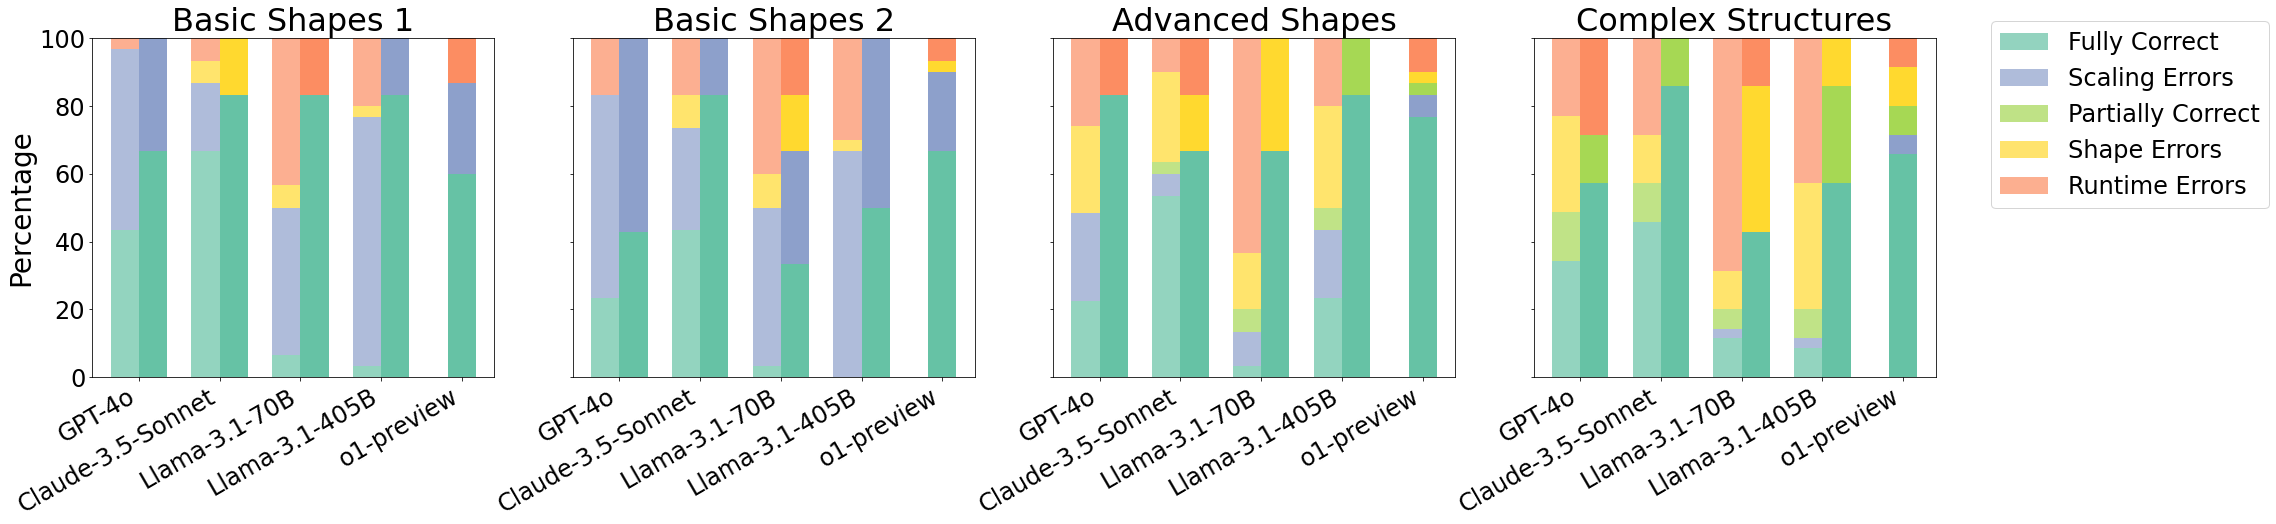
\includegraphics[width=\textwidth]{output.png}
  \caption{Baseline LLM Performance on Layout Design Tasks}
  \label{fig:baseline-llm-performance}
\end{figure}
The results reveal several common mistakes and limitations of standalone LLMs in handling layout design tasks:

1. \textbf{Scaling errors}: LLMs often struggled with unit conversion, failing to scale shapes from millimeters to micrometers (gdspy's default unit). This issue was particularly prevalent in Llama-3 models as can be seen from the dark blue ``Wrong Scale'' part of bar chart. They sometimes even assumed the user had made a mistake by requesting millimeters, and proceeded to 
draw in micrometers instead, justifying this choice 
with comments like "not mm, as the GDSII format is 
micrometers". This type of ``arrogant'' behavior and 
misalignment with human instructions on simple tasks 
will be very harmful for deploying LLMs as fully 
automanous AI agents. A recent Nature paper \cite
{ZhouNature2024} has also discussed similar 
observations. (see Appendix \ref{appendix:scaling_errors} for detailed examples).

2. \textbf{Partial correctness}: In complex tasks, LLMs sometimes generated partially correct results with right shapes but wrong relative positions.

3. \textbf{Shape errors}: Incorrect shapes often resulted from basic arithmetic errors, such as miscalculating angles for polygons (see Appendix \ref{appendix:shape_errors}). Many of these errors can be mitigated 
through Chain-of-Thought (CoT) prompting, which 
encourages the model to do calculations step-by-step.

4. \textbf{Runtime errors}: Approximately one-third of the generated code failed to execute due to various issues, including:
   - Attempts to use unavailable GUI features (particularly in GPT-4o and Claude-3.5-Sonnet)
   - Hallucinations of nonexistent gdspy functions
   - Typical programming logic mistakes
   (See Appendix \ref{appendix:runtime_errors} for a detailed error report)

5. \textbf{Inefficient code}: In one particular case, the Llama-3.1-405B model generated code with excessive object creation and boolean operations, leading to high memory usage and extended execution times (see Appendix \ref{appendix:inefficient_code} for the DLDChip task example).

6. \textbf{Ambiguous instructions}: When prompts could be interpreted in multiple ways, LLMs sometimes produced divergent results, highlighting the need for clear and specific instructions (see Appendix \ref{appendix:ambiguous_instructions} for examples).

Many of these issues can be mitigated by augmenting the LLMs with more advanced setup. Specifically, using Retrieval-Augmented Generation (RAG) to provide gdspy documentation to the LLMs, we should be able to reduce the errors related to misspelling and hallucinating nonexistent functions. For complex tasks, we can provide example code of simple shapes for In-Context Learning, so the LLMs only need to reason about positioning and scaling, and avoid runtime errors. We will discuss more in Section 3.

\section{Multimodal Inputs and Spatial Reasoning}
Layout design in semiconductor processes requires not only generating correct basic geometric shapes but also spatial reasoning to create proper ``layouts'' that meet specific requirements. Via connections, which create electrical pathways between different chip layers, exemplify this challenge. While seemingly simple—typically consisting of circular vias and rectangular metal connections—they demand precise positioning and sizing to ensure no short or open circuits and other functionality issues.

We conducted a series of tests by providing a sketch(image) together with different text prompts. The sketch are color-coded to represent different layers (e.g., yellow for via, blue for metal, red for pad) to help LLM understand the spatial relationships. We varied the text prompts to test the LLMs' spatial reasoning. We used GPT-4o's vision input capability for this experiment. Figure \ref{fig:via_experiment} illustrates the sketch inputs and corresponding LLM-generated outputs for each test case.
\begin{figure}[h]
\centering
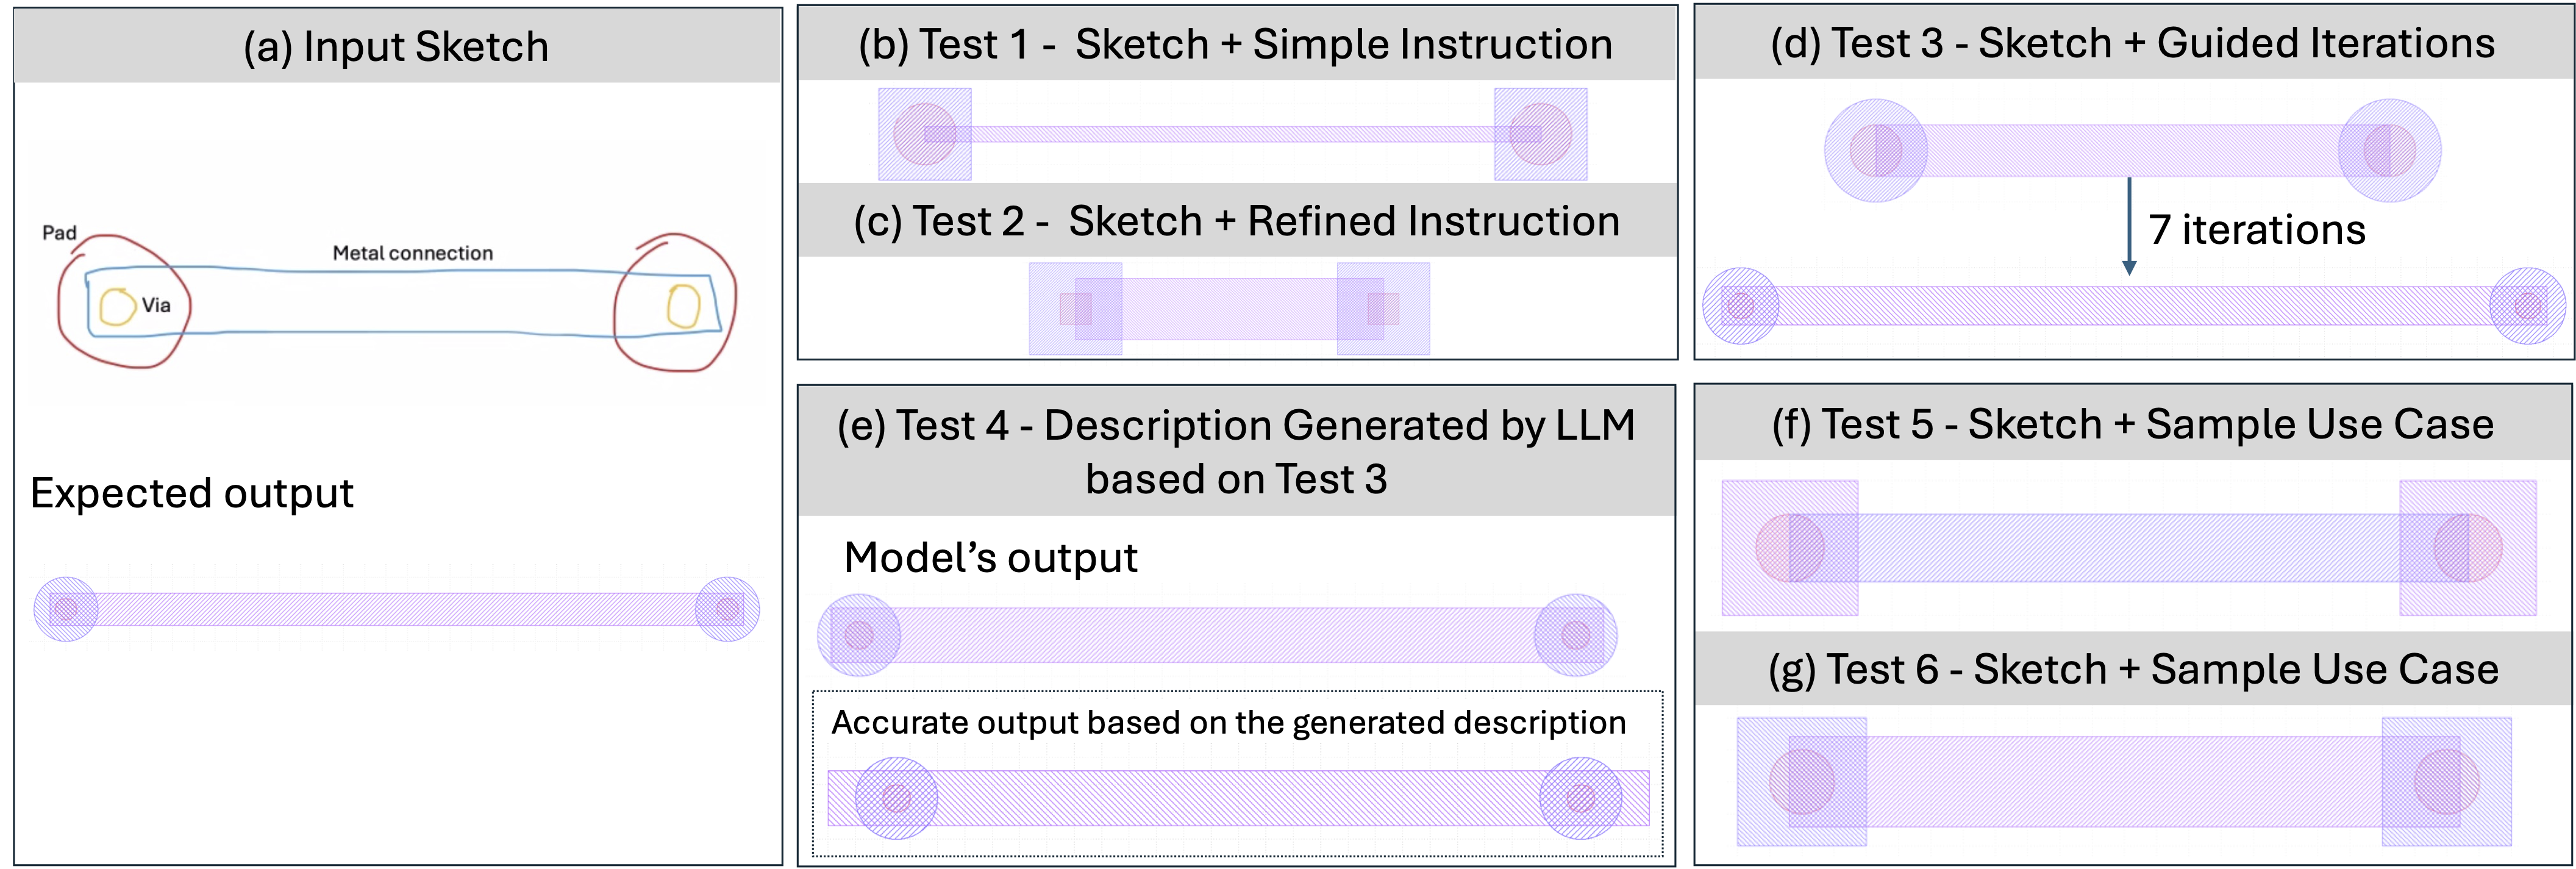
\includegraphics[width=0.8\textwidth]{Figure1_v5.png}
\caption{Sketch input and LLM-generated outputs for the via connection experiment. The sketch depicts a desired layout with two vias connected by a metal layer and circular pads on top. The outputs show the progression of the LLM's understanding and refinement of the layout based on iterative feedback and context provided by the user.}
\label{fig:via_experiment}
\end{figure}
In \textbf{Test 1}, we provided a basic sketch (Figure ~\ref{fig:via_experiment}(a)) with simple instructions. The LLM generated code, but the output had issues, including insufficient metal connection width. \textbf{Test 2} involved refining the description, but the output incorrectly used square vias and pads, and failed to properly cover the vias with metal. In \textbf{Test 3}, we provided a more detailed description. After seven iterations of feedback, the LLM finally produced the correct layout (Figure ~\ref{fig:via_experiment}(d)). See Appendix \ref{appendix:via_connection} for detailed prompts and the iterative process.

\textbf{Test 4} reversed the process by asking the LLM to create a detailed prompt based on the correct layout from \textbf{Test 3} (Appendix \ref{appendix:via_connection}). The LLM described each component's size and location in detail but hallucinated an additional requirement: \textit{a 50-unit space between the vias and the edges of the metal connection}. This would result in the layout shown in the dotted rectangle in Figure~\ref{fig:via_experiment}(e), where the metal extends beyond the contact pad. Interestingly, when given this ``wrong'' prompt, GPT-4o ignored the added specification and produced a layout matching the original design, with the metal not extending beyond the pad. Code inspection revealed that the LLM used another requirement, \textit{Leave a margin of 10 units between the edge of the metal and the pads}, to calculate the metal edge position in both x and y directions, although this was intended only for the y-direction margin. Using this version of prompt in the baseline evaluations (Section 1), o1-preview and Llama-3.1-405B each produced the ``non-extending'' version in one out of 5 runs, indicating some ambiguity in the specification. Generally, providing specific numerical values for size and location of geometric shapes in the prompt proves more robust than simple instructions like ``draw me a via''.

To further test our hypothesis, we conducted \textbf{Tests 5} and \textbf{6}, removing numerical values from the prompt and incorporating domain-specific context (e.g., 3D packaging and Through-Silicon Vias). This approach, however, degraded LLM performance, revealing a critical limitation: while LLMs possess textbook knowledge of semiconductor concepts, they struggle to translate this into practical design requirements. For instance, LLMs failed to apply common engineering knowledge, such as using wider metal layers to connect vias or leaving margin space between components in different layers to account for layermisalignment.

This finding underscores the importance of improving LLMs' reasoning capability of applying domain knowledge in problem-solving, rather than simply increasing model size to remember more knowledge, to enhance the adaptability of LLM-based AI systems.

\section{Neuro-inspired LLM Reasoning Network Architecture}

Based on our observations, we hypothesize that LLMs' poor performance in layout design tasks stems from weak spatial reasoning and difficulty applying domain knowledge.

To test this hypothesis, we employed our proprietary System for Optimizing Language Outputs through Multi-agent Oversight Networks (SOLOMON). Originally developed as part of a grant proposal for the ARPA-H ADVANCED RESEARCH PROJECTS AGENCY FOR HEALTH CHATBOT ACCURACY AND RELIABILITY EVALUATION (CARE) EXPLORATION TOPIC, SOLOMON was designed to detect and correct LLM hallucinations in healthcare applications. The system is based on a Neuro-inspired LLM Reasoning Network Architecture, drawing inspiration from Brain-like AGI \cite{Byrnes2022} and the Free Energy Principle (FEP) theory \cite{Parr2022}.

At its core, SOLOMON's key innovation lies in its multi-layered approach: 
(1) Thought Generators: A pool of multiple LLMs, each with distinct knowledge bases and reasoning abilities, trained on diverse datasets and fine-tuned for specific instruction-following capabilities. This approach can be seen as an effective parallel search through the Tree-of-Thoughts \cite{yao2023treethoughtsdeliberateproblem, zhang2024cumulativereasoninglargelanguage, Besta_2024, besta2024demystifyingchainstreesgraphs}, avoiding the bias problems associated with single LLM Chain-of-Thoughts approach. For instance, as observed in our scaling errors (see Appendix \ref{appendix:scaling_errors}), different LLM families exhibited distinct biases in unit interpretation.
(2) Thought Assessor: An LLM-based system leveraging the Free Energy Principle to analyze consensus and differences among proposed "Thoughts". This component enhances the LLM-as-a-Judge method \cite{zheng2023judgingllmasajudgemtbenchchatbot, guerreiro2023lookingneedlehaystackcomprehensive, lin2023llmevalunifiedmultidimensionalautomatic, ji2023mitigatinghallucinationlargelanguage} by incorporating the Free Energy Principle for more robust assessment.
(3) Steering Subsystem: Currently human-operated, this component provides instructions to guide the Thought Assessor in generating the final output.

This architecture enables SOLOMON to combine diverse perspectives, assess their validity, and produce a refined output, potentially mitigating individual LLM limitations in spatial reasoning and domain knowledge application.
\begin{figure}[h]
  \centering
  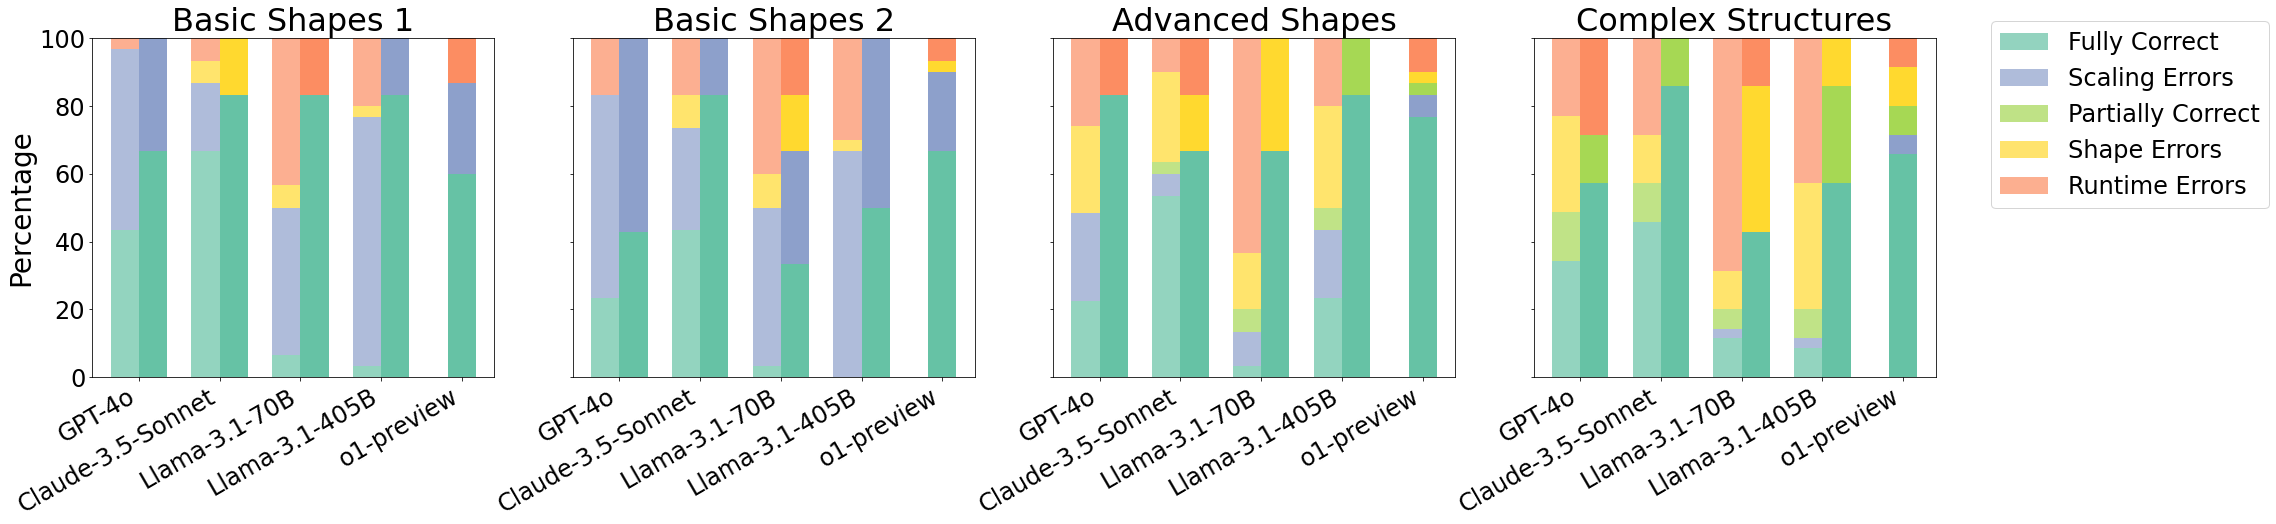
\includegraphics[width=\textwidth]{output.png}
  \caption{Performance comparison between 4 instances of SOLOMON built with classic non-reasoning LLMs versus o1-preview, the SOTA of reasoning LLM.}
  \label{fig:judges-performance}
\end{figure}
Figure \ref{fig:judges-performance} shows SOLOMON's performance on the same 25 tasks. We used 20 "Thoughts" from GPT-4o, Claude, and two Llama-3.1 models, including code, error reports, and rendered GDSII images (for GPT-4o and Claude only). We created 4 SOLOMON instances, each using one of the 4 LLMs as a Thought Assessor. The o1-preview result is shown side-by-side for comparison purposes only, its output is not used in SOLOMON's pool of thoughts.

Performance improved for all 4 LLMs compared to their baseline, with runtime errors almost completely eliminated. Improvement was more significant for GPT-4o and Claude due to their vision input capability, which assists spatial reasoning. Without vision input, Llama-3.1 models could only avoid runtime errors but struggled to evaluate spatial layouts effectively. We can see that SOLOMON's performance is comparable to o1-preview, the SOTA of reasoning LLM.

\section{Conclusion and Future Work}
The introduction of the SOLOMON architecture significantly improved performance, particularly in reducing runtime errors and enhancing spatial reasoning capabilities. However, challenges remain in translating domain knowledge into practical design requirements.

Future research directions include:
(1) Creating comprehensive benchmarks for LLM capabilities in layout design tasks.
(2) Exploring more configurations of SOLOMON architecture to understand the interaction between quality of initial thoughts vs assessment by ensemble, i.e., system 1 vs system 2 contributions in reasoning tasks.
(3) Exploring stacking layers of SOLOMON architecture to form a hierarchical reasoning model, for recalling and reasoning domain knowledge for solving the task on hand.
(4) Exploring the adaptability of SOLOMON architecture across different domains.

While LLMs show promise as layout design copilots, further advancements in reasoning capabilities and domain knowledge application are necessary for their effective integration into semiconductor design processes and other domain specific tasks.

\textbf{Acknowledgment:} We thank Kuan Yu Hsieh for her valuable contribution in creating the dataset of 25 tasks with ground truth and her exploration work on the via connection test cases.

\bibliographystyle{plainnat}
\bibliography{bibliography}

% Add the NeurIPS Paper Checklist here, before any supplementary material
\newpage
\section*{Checklist}


\begin{enumerate}

    \item {\bf Claims}
        \item[] Question: Do the main claims made in the abstract and introduction accurately reflect the paper's contributions and scope?
        \item[] Answer: \answerTODO{} % Replace by \answerYes{}, \answerNo{}, or \answerNA{}.
        \item[] Justification: \justificationTODO{}
        \item[] Guidelines:
        \begin{itemize}
            \item The answer NA means that the abstract and introduction do not include the claims made in the paper.
            \item The abstract and/or introduction should clearly state the claims made, including the contributions made in the paper and important assumptions and limitations. A No or NA answer to this question will not be perceived well by the reviewers. 
            \item The claims made should match theoretical and experimental results, and reflect how much the results can be expected to generalize to other settings. 
            \item It is fine to include aspirational goals as motivation as long as it is clear that these goals are not attained by the paper. 
        \end{itemize}
    
    \item {\bf Limitations}
        \item[] Question: Does the paper discuss the limitations of the work performed by the authors?
        \item[] Answer: \answerTODO{} % Replace by \answerYes{}, \answerNo{}, or \answerNA{}.
        \item[] Justification: \justificationTODO{}
        \item[] Guidelines:
        \begin{itemize}
            \item The answer NA means that the paper has no limitation while the answer No means that the paper has limitations, but those are not discussed in the paper. 
            \item The authors are encouraged to create a separate "Limitations" section in their paper.
            \item The paper should point out any strong assumptions and how robust the results are to violations of these assumptions (e.g., independence assumptions, noiseless settings, model well-specification, asymptotic approximations only holding locally). The authors should reflect on how these assumptions might be violated in practice and what the implications would be.
            \item The authors should reflect on the scope of the claims made, e.g., if the approach was only tested on a few datasets or with a few runs. In general, empirical results often depend on implicit assumptions, which should be articulated.
            \item The authors should reflect on the factors that influence the performance of the approach. For example, a facial recognition algorithm may perform poorly when image resolution is low or images are taken in low lighting. Or a speech-to-text system might not be used reliably to provide closed captions for online lectures because it fails to handle technical jargon.
            \item The authors should discuss the computational efficiency of the proposed algorithms and how they scale with dataset size.
            \item If applicable, the authors should discuss possible limitations of their approach to address problems of privacy and fairness.
            \item While the authors might fear that complete honesty about limitations might be used by reviewers as grounds for rejection, a worse outcome might be that reviewers discover limitations that aren't acknowledged in the paper. The authors should use their best judgment and recognize that individual actions in favor of transparency play an important role in developing norms that preserve the integrity of the community. Reviewers will be specifically instructed to not penalize honesty concerning limitations.
        \end{itemize}
    
    \item {\bf Theory Assumptions and Proofs}
        \item[] Question: For each theoretical result, does the paper provide the full set of assumptions and a complete (and correct) proof?
        \item[] Answer: \answerTODO{} % Replace by \answerYes{}, \answerNo{}, or \answerNA{}.
        \item[] Justification: \justificationTODO{}
        \item[] Guidelines:
        \begin{itemize}
            \item The answer NA means that the paper does not include theoretical results. 
            \item All the theorems, formulas, and proofs in the paper should be numbered and cross-referenced.
            \item All assumptions should be clearly stated or referenced in the statement of any theorems.
            \item The proofs can either appear in the main paper or the supplemental material, but if they appear in the supplemental material, the authors are encouraged to provide a short proof sketch to provide intuition. 
            \item Inversely, any informal proof provided in the core of the paper should be complemented by formal proofs provided in appendix or supplemental material.
            \item Theorems and Lemmas that the proof relies upon should be properly referenced. 
        \end{itemize}
    
        \item {\bf Experimental Result Reproducibility}
        \item[] Question: Does the paper fully disclose all the information needed to reproduce the main experimental results of the paper to the extent that it affects the main claims and/or conclusions of the paper (regardless of whether the code and data are provided or not)?
        \item[] Answer: \answerTODO{} % Replace by \answerYes{}, \answerNo{}, or \answerNA{}.
        \item[] Justification: \justificationTODO{}
        \item[] Guidelines:
        \begin{itemize}
            \item The answer NA means that the paper does not include experiments.
            \item If the paper includes experiments, a No answer to this question will not be perceived well by the reviewers: Making the paper reproducible is important, regardless of whether the code and data are provided or not.
            \item If the contribution is a dataset and/or model, the authors should describe the steps taken to make their results reproducible or verifiable. 
            \item Depending on the contribution, reproducibility can be accomplished in various ways. For example, if the contribution is a novel architecture, describing the architecture fully might suffice, or if the contribution is a specific model and empirical evaluation, it may be necessary to either make it possible for others to replicate the model with the same dataset, or provide access to the model. In general. releasing code and data is often one good way to accomplish this, but reproducibility can also be provided via detailed instructions for how to replicate the results, access to a hosted model (e.g., in the case of a large language model), releasing of a model checkpoint, or other means that are appropriate to the research performed.
            \item While NeurIPS does not require releasing code, the conference does require all submissions to provide some reasonable avenue for reproducibility, which may depend on the nature of the contribution. For example
            \begin{enumerate}
                \item If the contribution is primarily a new algorithm, the paper should make it clear how to reproduce that algorithm.
                \item If the contribution is primarily a new model architecture, the paper should describe the architecture clearly and fully.
                \item If the contribution is a new model (e.g., a large language model), then there should either be a way to access this model for reproducing the results or a way to reproduce the model (e.g., with an open-source dataset or instructions for how to construct the dataset).
                \item We recognize that reproducibility may be tricky in some cases, in which case authors are welcome to describe the particular way they provide for reproducibility. In the case of closed-source models, it may be that access to the model is limited in some way (e.g., to registered users), but it should be possible for other researchers to have some path to reproducing or verifying the results.
            \end{enumerate}
        \end{itemize}
    
    
    \item {\bf Open access to data and code}
        \item[] Question: Does the paper provide open access to the data and code, with sufficient instructions to faithfully reproduce the main experimental results, as described in supplemental material?
        \item[] Answer: \answerTODO{} % Replace by \answerYes{}, \answerNo{}, or \answerNA{}.
        \item[] Justification: \justificationTODO{}
        \item[] Guidelines:
        \begin{itemize}
            \item The answer NA means that paper does not include experiments requiring code.
            \item Please see the NeurIPS code and data submission guidelines (\url{https://nips.cc/public/guides/CodeSubmissionPolicy}) for more details.
            \item While we encourage the release of code and data, we understand that this might not be possible, so “No” is an acceptable answer. Papers cannot be rejected simply for not including code, unless this is central to the contribution (e.g., for a new open-source benchmark).
            \item The instructions should contain the exact command and environment needed to run to reproduce the results. See the NeurIPS code and data submission guidelines (\url{https://nips.cc/public/guides/CodeSubmissionPolicy}) for more details.
            \item The authors should provide instructions on data access and preparation, including how to access the raw data, preprocessed data, intermediate data, and generated data, etc.
            \item The authors should provide scripts to reproduce all experimental results for the new proposed method and baselines. If only a subset of experiments are reproducible, they should state which ones are omitted from the script and why.
            \item At submission time, to preserve anonymity, the authors should release anonymized versions (if applicable).
            \item Providing as much information as possible in supplemental material (appended to the paper) is recommended, but including URLs to data and code is permitted.
        \end{itemize}
    
    
    \item {\bf Experimental Setting/Details}
        \item[] Question: Does the paper specify all the training and test details (e.g., data splits, hyperparameters, how they were chosen, type of optimizer, etc.) necessary to understand the results?
        \item[] Answer: \answerTODO{} % Replace by \answerYes{}, \answerNo{}, or \answerNA{}.
        \item[] Justification: \justificationTODO{}
        \item[] Guidelines:
        \begin{itemize}
            \item The answer NA means that the paper does not include experiments.
            \item The experimental setting should be presented in the core of the paper to a level of detail that is necessary to appreciate the results and make sense of them.
            \item The full details can be provided either with the code, in appendix, or as supplemental material.
        \end{itemize}
    
    \item {\bf Experiment Statistical Significance}
        \item[] Question: Does the paper report error bars suitably and correctly defined or other appropriate information about the statistical significance of the experiments?
        \item[] Answer: \answerTODO{} % Replace by \answerYes{}, \answerNo{}, or \answerNA{}.
        \item[] Justification: \justificationTODO{}
        \item[] Guidelines:
        \begin{itemize}
            \item The answer NA means that the paper does not include experiments.
            \item The authors should answer "Yes" if the results are accompanied by error bars, confidence intervals, or statistical significance tests, at least for the experiments that support the main claims of the paper.
            \item The factors of variability that the error bars are capturing should be clearly stated (for example, train/test split, initialization, random drawing of some parameter, or overall run with given experimental conditions).
            \item The method for calculating the error bars should be explained (closed form formula, call to a library function, bootstrap, etc.)
            \item The assumptions made should be given (e.g., Normally distributed errors).
            \item It should be clear whether the error bar is the standard deviation or the standard error of the mean.
            \item It is OK to report 1-sigma error bars, but one should state it. The authors should preferably report a 2-sigma error bar than state that they have a 96\% CI, if the hypothesis of Normality of errors is not verified.
            \item For asymmetric distributions, the authors should be careful not to show in tables or figures symmetric error bars that would yield results that are out of range (e.g. negative error rates).
            \item If error bars are reported in tables or plots, The authors should explain in the text how they were calculated and reference the corresponding figures or tables in the text.
        \end{itemize}
    
    \item {\bf Experiments Compute Resources}
        \item[] Question: For each experiment, does the paper provide sufficient information on the computer resources (type of compute workers, memory, time of execution) needed to reproduce the experiments?
        \item[] Answer: \answerTODO{} % Replace by \answerYes{}, \answerNo{}, or \answerNA{}.
        \item[] Justification: \justificationTODO{}
        \item[] Guidelines:
        \begin{itemize}
            \item The answer NA means that the paper does not include experiments.
            \item The paper should indicate the type of compute workers CPU or GPU, internal cluster, or cloud provider, including relevant memory and storage.
            \item The paper should provide the amount of compute required for each of the individual experimental runs as well as estimate the total compute. 
            \item The paper should disclose whether the full research project required more compute than the experiments reported in the paper (e.g., preliminary or failed experiments that didn't make it into the paper). 
        \end{itemize}
        
    \item {\bf Code Of Ethics}
        \item[] Question: Does the research conducted in the paper conform, in every respect, with the NeurIPS Code of Ethics \url{https://neurips.cc/public/EthicsGuidelines}?
        \item[] Answer: \answerTODO{} % Replace by \answerYes{}, \answerNo{}, or \answerNA{}.
        \item[] Justification: \justificationTODO{}
        \item[] Guidelines:
        \begin{itemize}
            \item The answer NA means that the authors have not reviewed the NeurIPS Code of Ethics.
            \item If the authors answer No, they should explain the special circumstances that require a deviation from the Code of Ethics.
            \item The authors should make sure to preserve anonymity (e.g., if there is a special consideration due to laws or regulations in their jurisdiction).
        \end{itemize}
    
    
    \item {\bf Broader Impacts}
        \item[] Question: Does the paper discuss both potential positive societal impacts and negative societal impacts of the work performed?
        \item[] Answer: \answerTODO{} % Replace by \answerYes{}, \answerNo{}, or \answerNA{}.
        \item[] Justification: \justificationTODO{}
        \item[] Guidelines:
        \begin{itemize}
            \item The answer NA means that there is no societal impact of the work performed.
            \item If the authors answer NA or No, they should explain why their work has no societal impact or why the paper does not address societal impact.
            \item Examples of negative societal impacts include potential malicious or unintended uses (e.g., disinformation, generating fake profiles, surveillance), fairness considerations (e.g., deployment of technologies that could make decisions that unfairly impact specific groups), privacy considerations, and security considerations.
            \item The conference expects that many papers will be foundational research and not tied to particular applications, let alone deployments. However, if there is a direct path to any negative applications, the authors should point it out. For example, it is legitimate to point out that an improvement in the quality of generative models could be used to generate deepfakes for disinformation. On the other hand, it is not needed to point out that a generic algorithm for optimizing neural networks could enable people to train models that generate Deepfakes faster.
            \item The authors should consider possible harms that could arise when the technology is being used as intended and functioning correctly, harms that could arise when the technology is being used as intended but gives incorrect results, and harms following from (intentional or unintentional) misuse of the technology.
            \item If there are negative societal impacts, the authors could also discuss possible mitigation strategies (e.g., gated release of models, providing defenses in addition to attacks, mechanisms for monitoring misuse, mechanisms to monitor how a system learns from feedback over time, improving the efficiency and accessibility of ML).
        \end{itemize}
        
    \item {\bf Safeguards}
        \item[] Question: Does the paper describe safeguards that have been put in place for responsible release of data or models that have a high risk for misuse (e.g., pretrained language models, image generators, or scraped datasets)?
        \item[] Answer: \answerTODO{} % Replace by \answerYes{}, \answerNo{}, or \answerNA{}.
        \item[] Justification: \justificationTODO{}
        \item[] Guidelines:
        \begin{itemize}
            \item The answer NA means that the paper poses no such risks.
            \item Released models that have a high risk for misuse or dual-use should be released with necessary safeguards to allow for controlled use of the model, for example by requiring that users adhere to usage guidelines or restrictions to access the model or implementing safety filters. 
            \item Datasets that have been scraped from the Internet could pose safety risks. The authors should describe how they avoided releasing unsafe images.
            \item We recognize that providing effective safeguards is challenging, and many papers do not require this, but we encourage authors to take this into account and make a best faith effort.
        \end{itemize}
    
    \item {\bf Licenses for existing assets}
        \item[] Question: Are the creators or original owners of assets (e.g., code, data, models), used in the paper, properly credited and are the license and terms of use explicitly mentioned and properly respected?
        \item[] Answer: \answerTODO{} % Replace by \answerYes{}, \answerNo{}, or \answerNA{}.
        \item[] Justification: \justificationTODO{}
        \item[] Guidelines:
        \begin{itemize}
            \item The answer NA means that the paper does not use existing assets.
            \item The authors should cite the original paper that produced the code package or dataset.
            \item The authors should state which version of the asset is used and, if possible, include a URL.
            \item The name of the license (e.g., CC-BY 4.0) should be included for each asset.
            \item For scraped data from a particular source (e.g., website), the copyright and terms of service of that source should be provided.
            \item If assets are released, the license, copyright information, and terms of use in the package should be provided. For popular datasets, \url{paperswithcode.com/datasets} has curated licenses for some datasets. Their licensing guide can help determine the license of a dataset.
            \item For existing datasets that are re-packaged, both the original license and the license of the derived asset (if it has changed) should be provided.
            \item If this information is not available online, the authors are encouraged to reach out to the asset's creators.
        \end{itemize}
    
    \item {\bf New Assets}
        \item[] Question: Are new assets introduced in the paper well documented and is the documentation provided alongside the assets?
        \item[] Answer: \answerTODO{} % Replace by \answerYes{}, \answerNo{}, or \answerNA{}.
        \item[] Justification: \justificationTODO{}
        \item[] Guidelines:
        \begin{itemize}
            \item The answer NA means that the paper does not release new assets.
            \item Researchers should communicate the details of the dataset/code/model as part of their submissions via structured templates. This includes details about training, license, limitations, etc. 
            \item The paper should discuss whether and how consent was obtained from people whose asset is used.
            \item At submission time, remember to anonymize your assets (if applicable). You can either create an anonymized URL or include an anonymized zip file.
        \end{itemize}
    
    \item {\bf Crowdsourcing and Research with Human Subjects}
        \item[] Question: For crowdsourcing experiments and research with human subjects, does the paper include the full text of instructions given to participants and screenshots, if applicable, as well as details about compensation (if any)? 
        \item[] Answer: \answerTODO{} % Replace by \answerYes{}, \answerNo{}, or \answerNA{}.
        \item[] Justification: \justificationTODO{}
        \item[] Guidelines:
        \begin{itemize}
            \item The answer NA means that the paper does not involve crowdsourcing nor research with human subjects.
            \item Including this information in the supplemental material is fine, but if the main contribution of the paper involves human subjects, then as much detail as possible should be included in the main paper. 
            \item According to the NeurIPS Code of Ethics, workers involved in data collection, curation, or other labor should be paid at least the minimum wage in the country of the data collector. 
        \end{itemize}
    
    \item {\bf Institutional Review Board (IRB) Approvals or Equivalent for Research with Human Subjects}
        \item[] Question: Does the paper describe potential risks incurred by study participants, whether such risks were disclosed to the subjects, and whether Institutional Review Board (IRB) approvals (or an equivalent approval/review based on the requirements of your country or institution) were obtained?
        \item[] Answer: \answerTODO{} % Replace by \answerYes{}, \answerNo{}, or \answerNA{}.
        \item[] Justification: \justificationTODO{}
        \item[] Guidelines:
        \begin{itemize}
            \item The answer NA means that the paper does not involve crowdsourcing nor research with human subjects.
            \item Depending on the country in which research is conducted, IRB approval (or equivalent) may be required for any human subjects research. If you obtained IRB approval, you should clearly state this in the paper. 
            \item We recognize that the procedures for this may vary significantly between institutions and locations, and we expect authors to adhere to the NeurIPS Code of Ethics and the guidelines for their institution. 
            \item For initial submissions, do not include any information that would break anonymity (if applicable), such as the institution conducting the review.
        \end{itemize}
    
    \end{enumerate}
    
    

\newpage
\appendix

\section{Appendix}
\subsection{Task Prompts and Baseline LLM Performance}
\label{appendix:task_prompts_and_performance}

This section presents the 25 tasks used in our evaluation, along with the performance of various LLMs and the SOLOMON system. For each task, we provide the prompt, the ground truth image, and a table showing the outputs from different LLMs across 5 runs, as well as the SOLOMON result.

The system prompt used for baseline experiment (thought generating) for all tasks was as follows:

\begin{verbatim}
You are an expert Python developer specialized in generating layout designs 
in GDS (GDSII) format. Your task is to assist the user in creating Python 
code that accurately draws layout designs while being mindful of the 
geometric relationships and layout accuracy.

Write down your thinking step by step before you start coding:
1. Always start by understanding the overall design requirements provided 
   by the user.
2. Break down the design into smaller components and define each geometric 
   shape with precise coordinates.
3. Ensure that all shapes and elements maintain their correct geometric 
   relationships, such as alignment, spacing, and proportional dimensions.
4. Validate each step of the design process to avoid errors and maintain 
   accuracy.

Use the 'gdspy' library to generate the GDS layout:
1. Parse the user's design specifications.
2. Define the library and cell for the GDS layout.
3. Create each geometric element (e.g., rectangles, polygons) with precise 
   coordinates.
4. Ensure elements are placed correctly and maintain their intended 
   relationships.
5. Save the design to a GDS file.

Provide all the code in a single ```python ``` block to the user without 
postamble. Do not include any other ``` block in your response to avoid 
parsing error in following steps.

Be meticulous in your approach, and always consider the geometric 
relationships and layout accuracy in every step of the design process.
\end{verbatim}

From table 1 to 5, we show selected examples from each category of tasks where the LLMs having trouble with the task.

% \begin{table}
  \caption{Arrow Task}
  \label{table:arrow}
  \centering
  \begin{tabularx}{\textwidth}{@{}XXXXXX@{}}
    \toprule
    \makecell{Ground Truth \\ 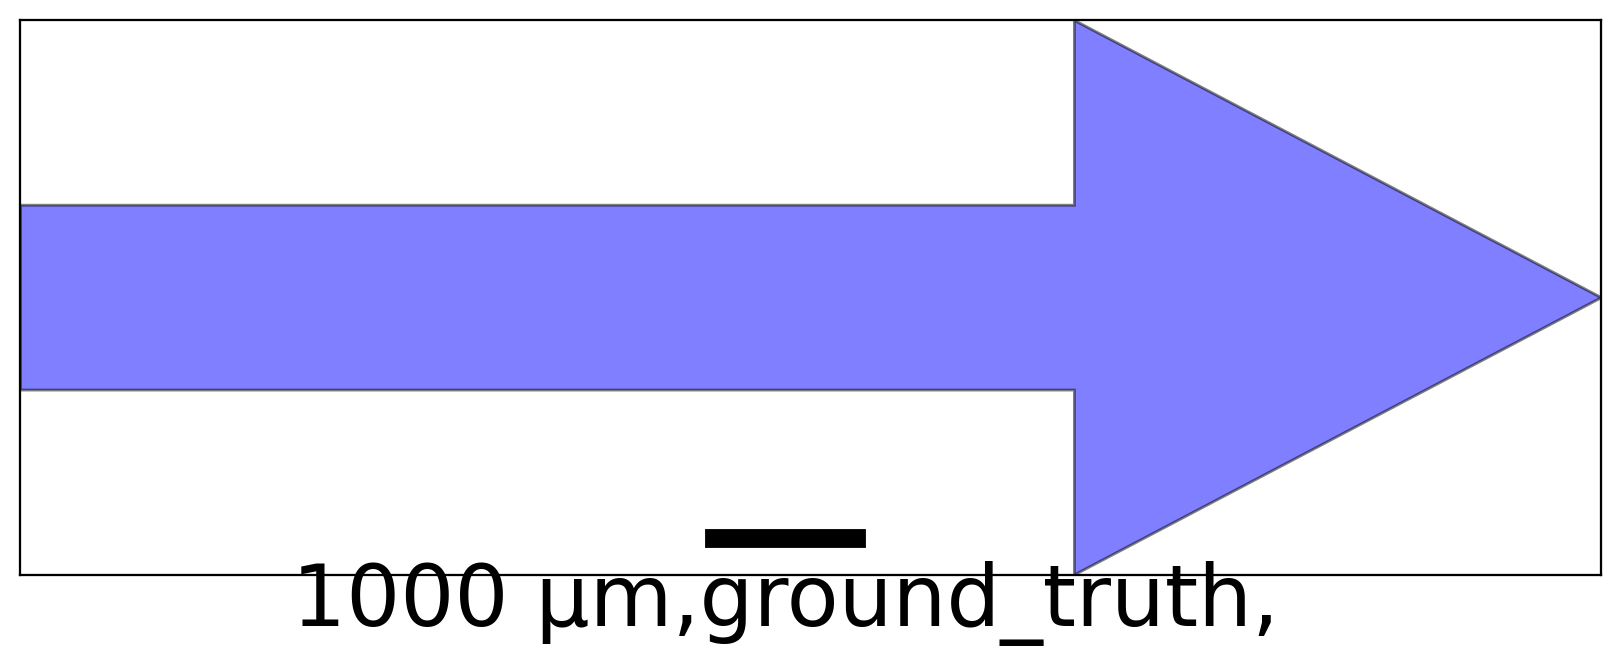
\includegraphics[width=0.13\textwidth]{examples_png/Arrow.png}} & GPT-4o & Claude-3.5 & Llama-3-70B & Llama-3-405B & o1-preview \\
    \midrule
    SOLOMON & 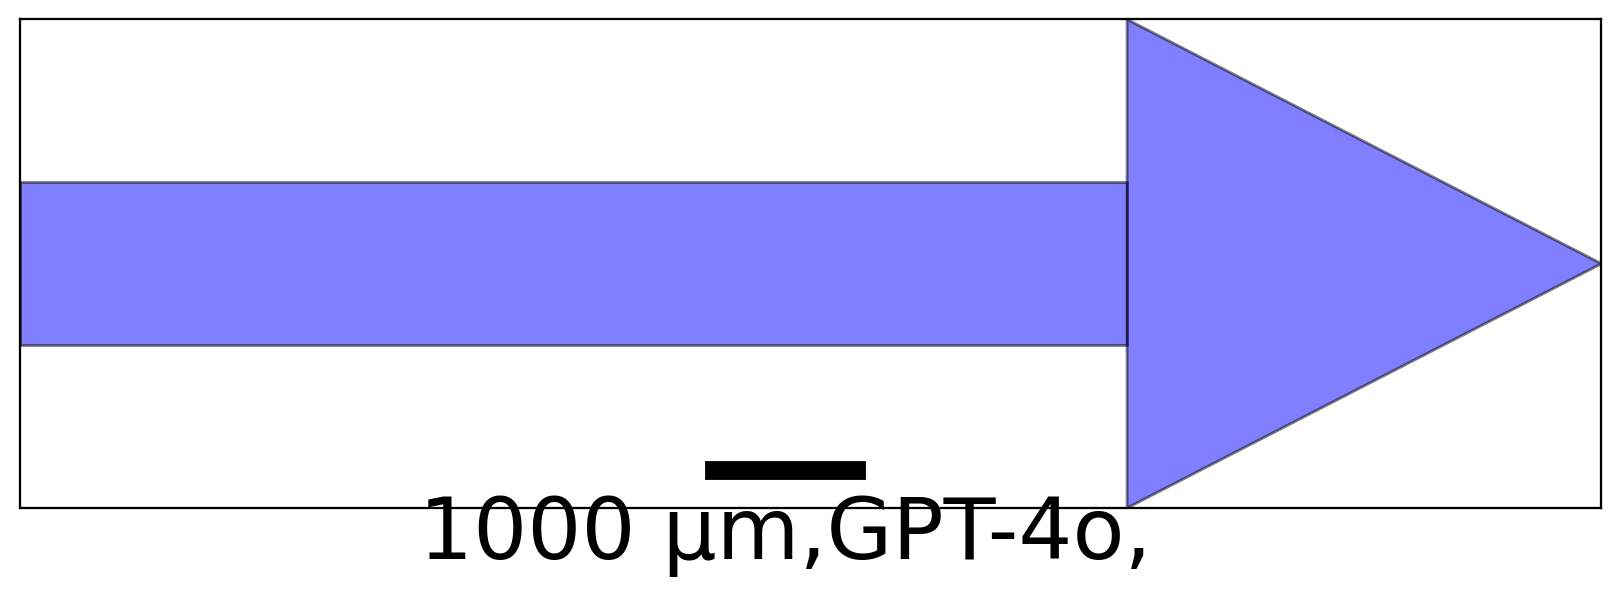
\includegraphics[width=0.13\textwidth]{./pool_all/png/gpt-4o_results/Arrow.png} &  & 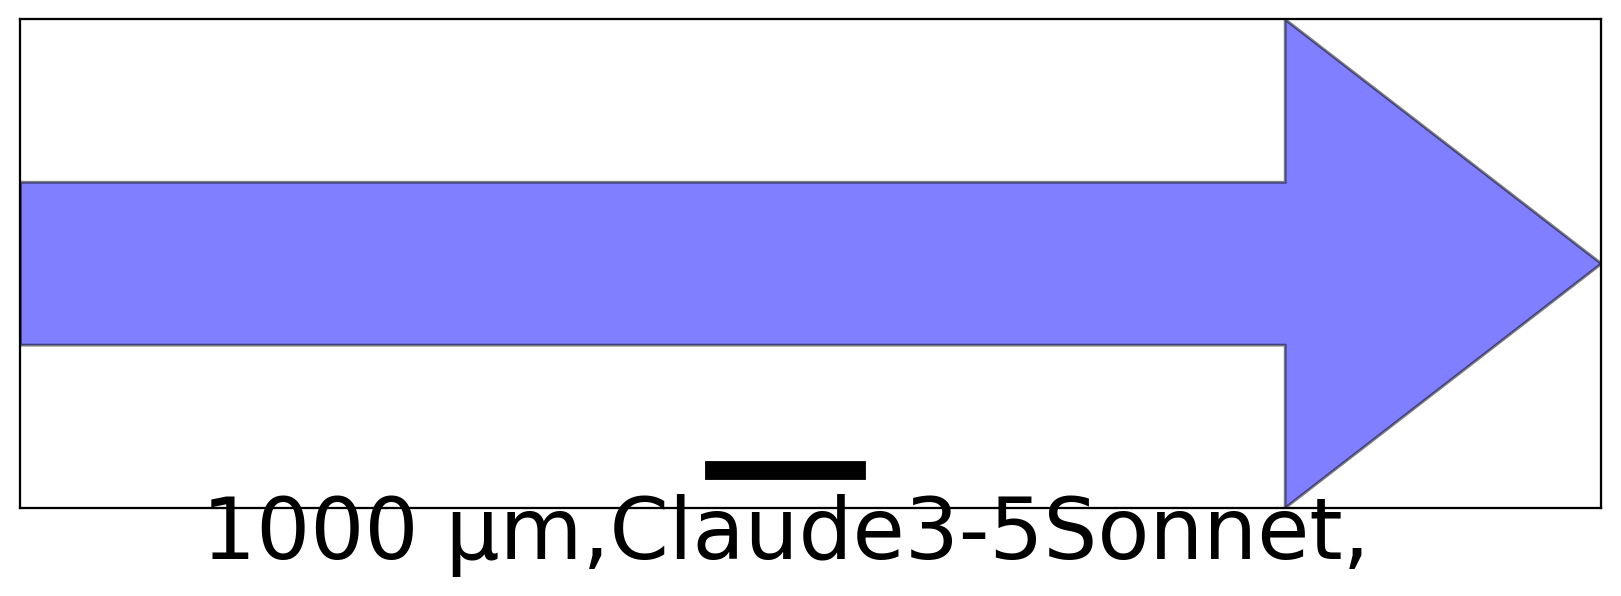
\includegraphics[width=0.13\textwidth]{./pool_all/png/claude-3-5-sonnet-20240620_results/Arrow.png} & 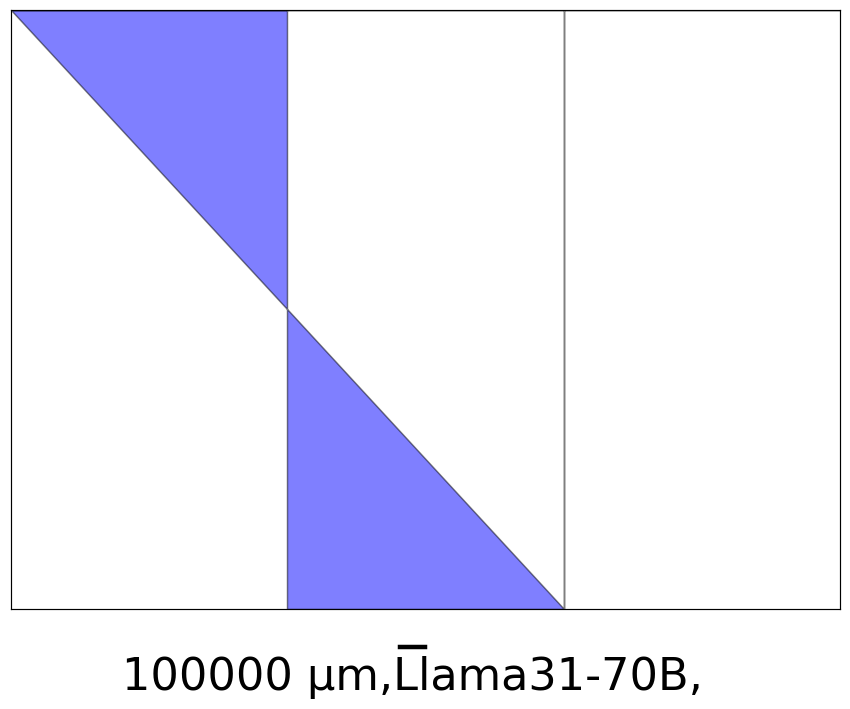
\includegraphics[width=0.13\textwidth]{./pool_all/png/watsonx_meta-llama_llama-3-1-70b-instruct_results/Arrow.png} & 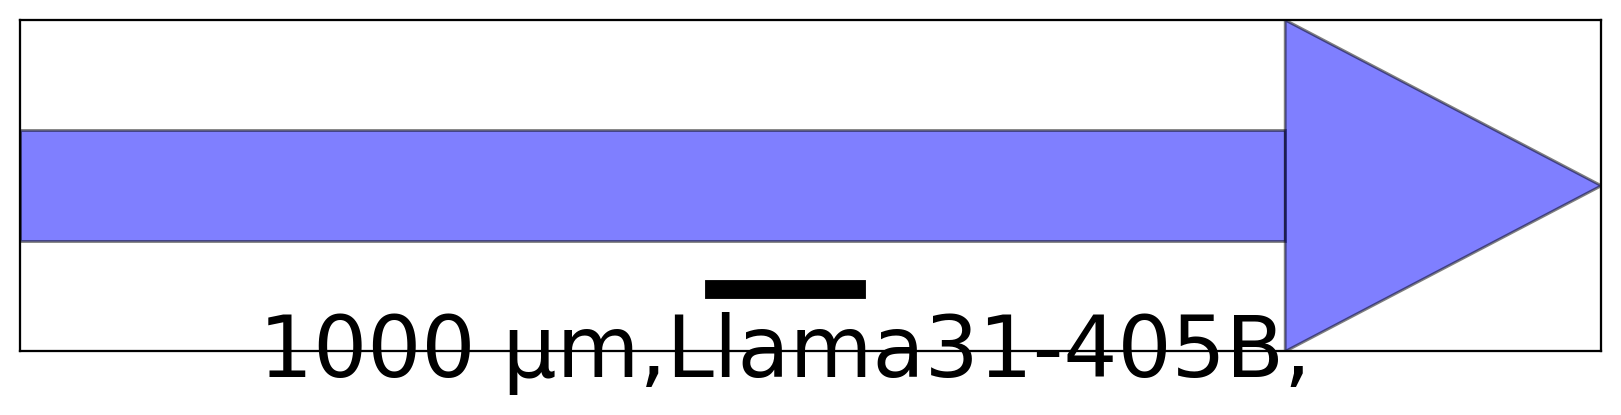
\includegraphics[width=0.13\textwidth]{./pool_all/png/watsonx_meta-llama_llama-3-405b-instruct_results/Arrow.png} \\
    \makecell{Single LLM \\ Baseline \\ Run 1} & 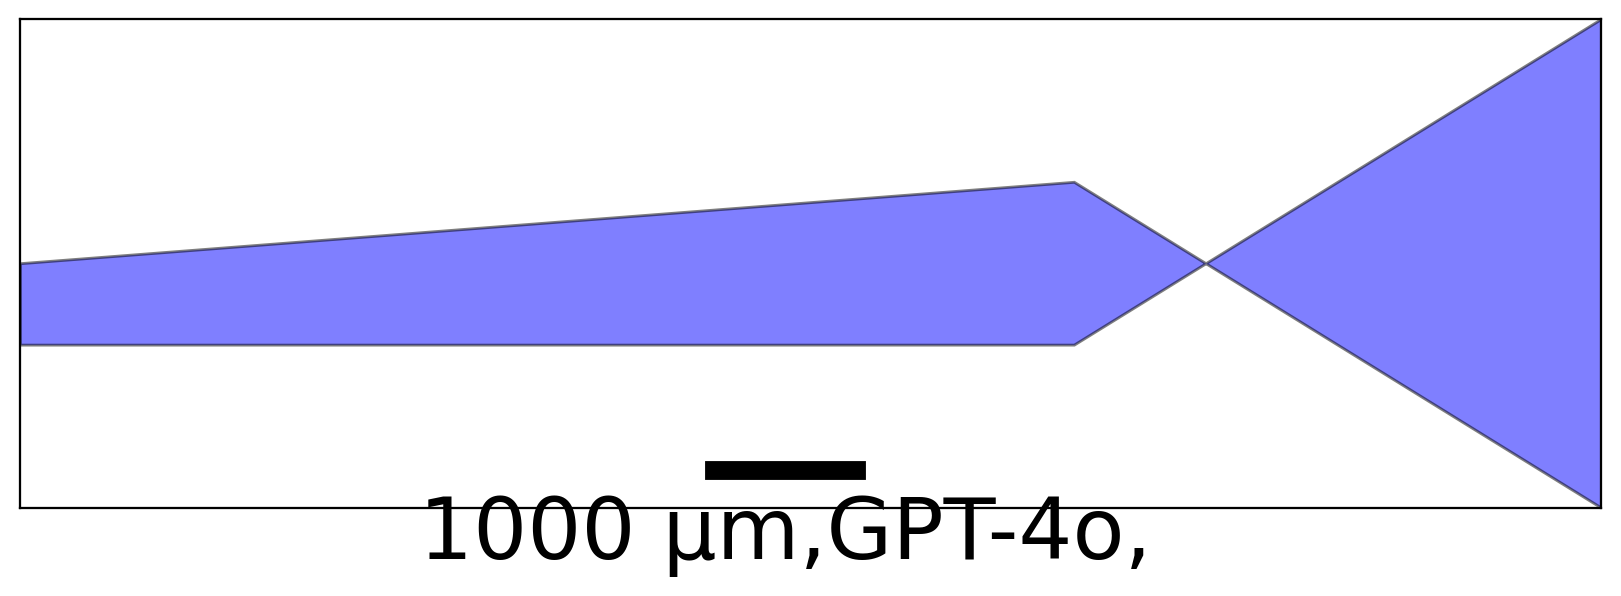
\includegraphics[width=0.13\textwidth]{./run_1/png/gpt-4o_results/Arrow.png} & 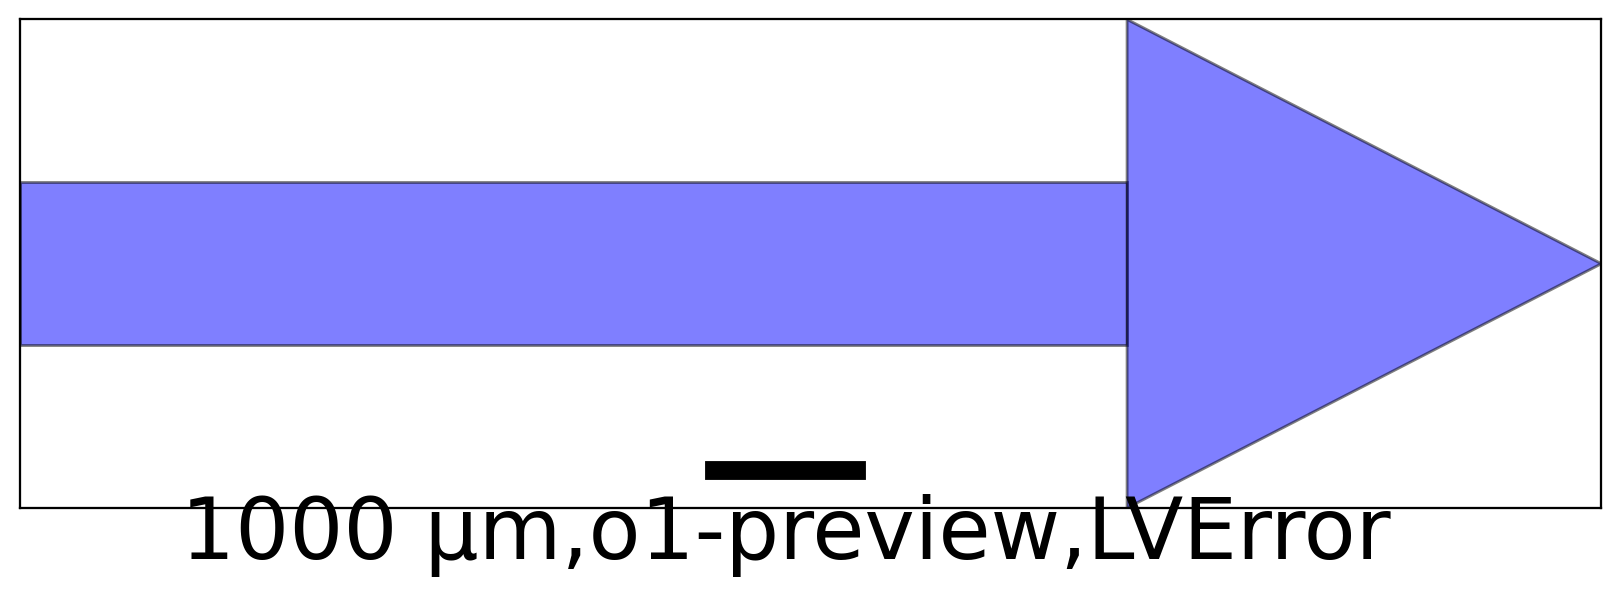
\includegraphics[width=0.13\textwidth]{./run_1/png/o1-preview_results/Arrow.png} & 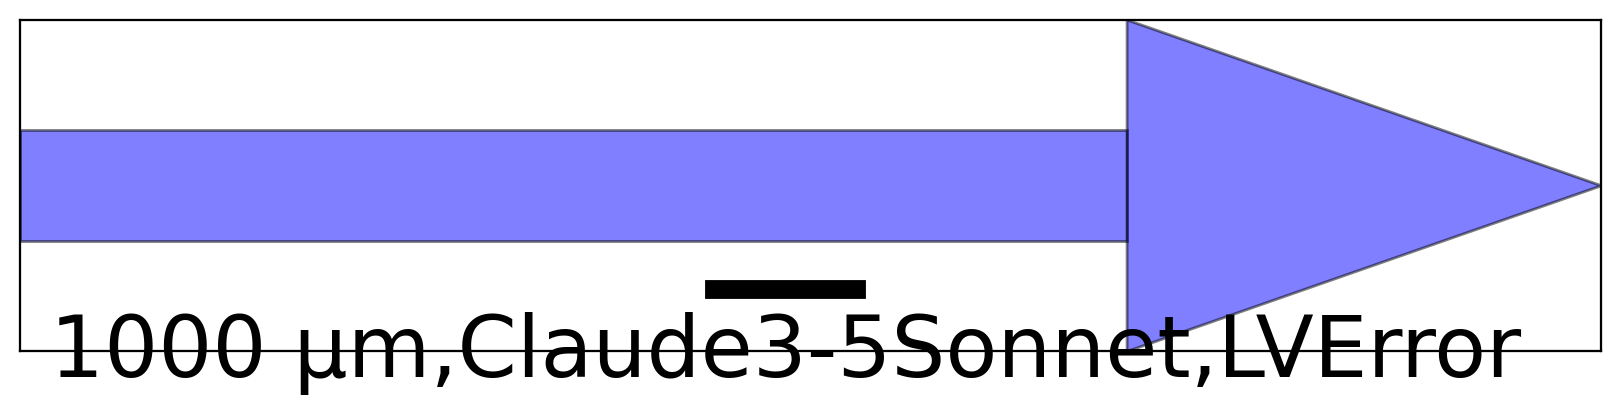
\includegraphics[width=0.13\textwidth]{./run_1/png/claude-3-5-sonnet-20240620_results/Arrow.png} & 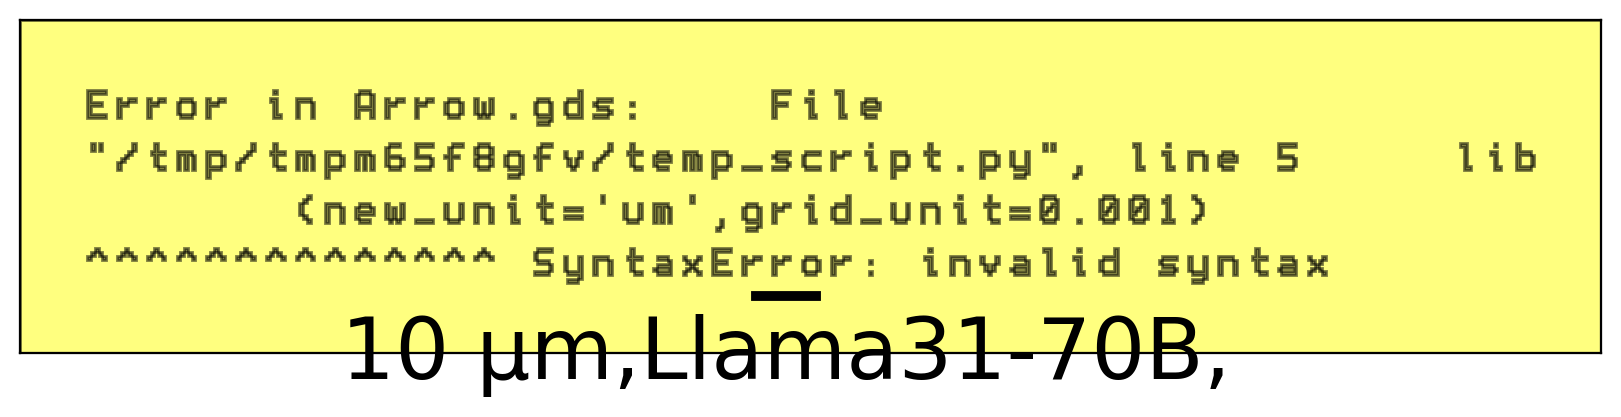
\includegraphics[width=0.13\textwidth]{./run_1/png/watsonx_meta-llama_llama-3-1-70b-instruct_results/Arrow.png} & 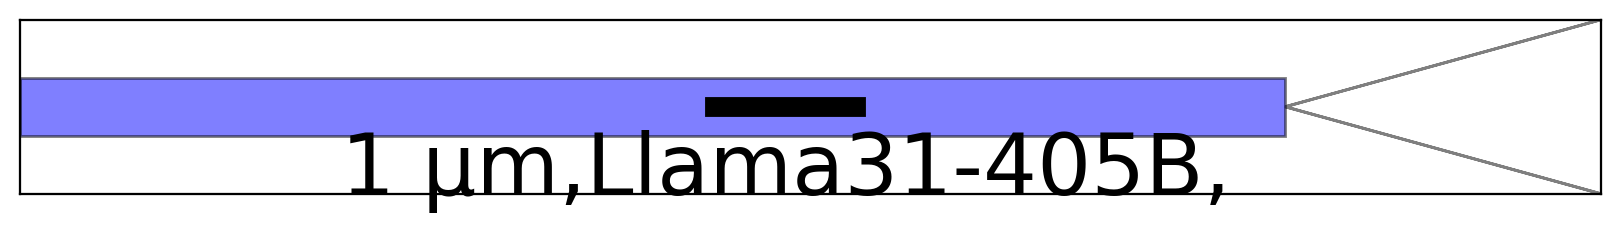
\includegraphics[width=0.13\textwidth]{./run_1/png/watsonx_meta-llama_llama-3-405b-instruct_results/Arrow.png} \\
    \makecell{Single LLM \\ Baseline \\ Run 2} & 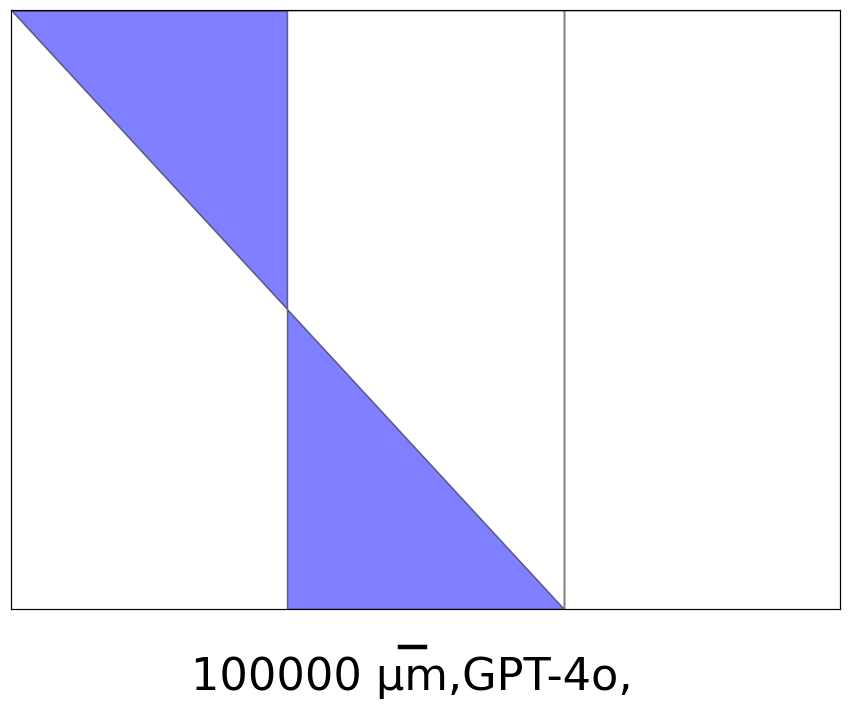
\includegraphics[width=0.13\textwidth]{./run_2/png/gpt-4o_results/Arrow.png} & 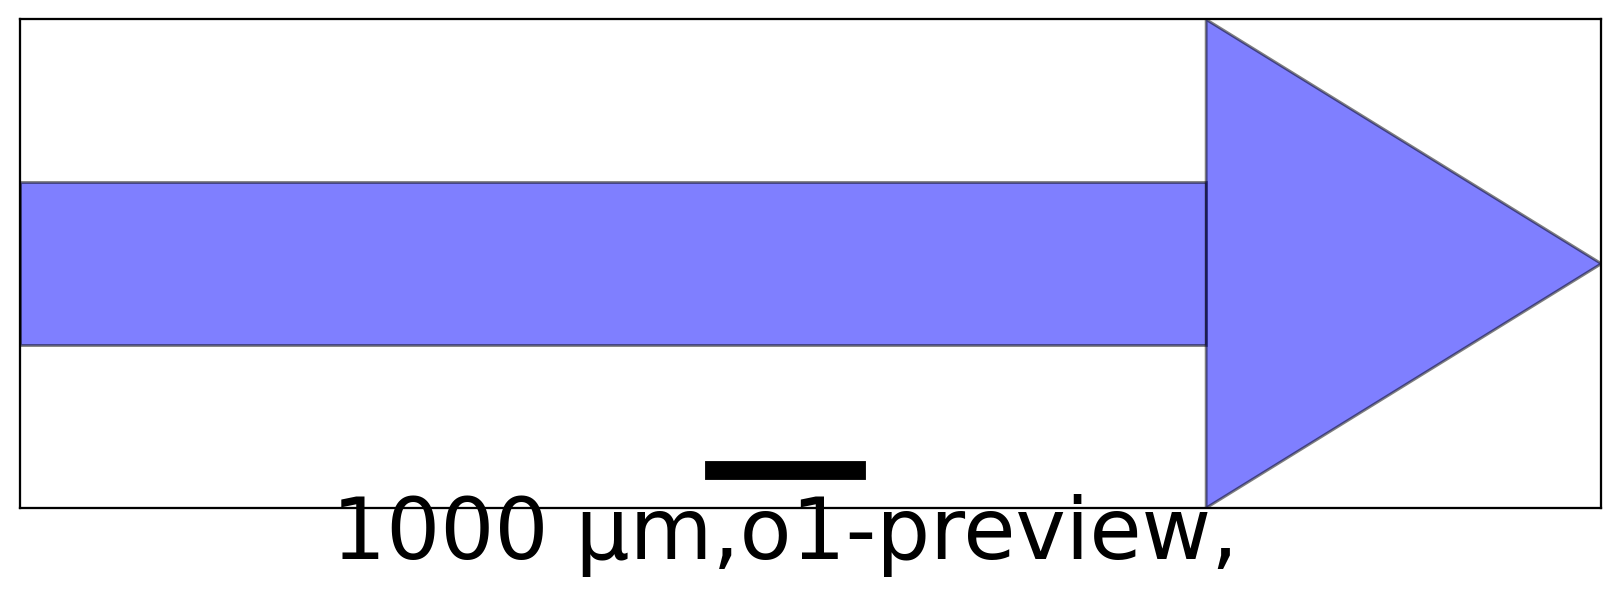
\includegraphics[width=0.13\textwidth]{./run_2/png/o1-preview_results/Arrow.png} & 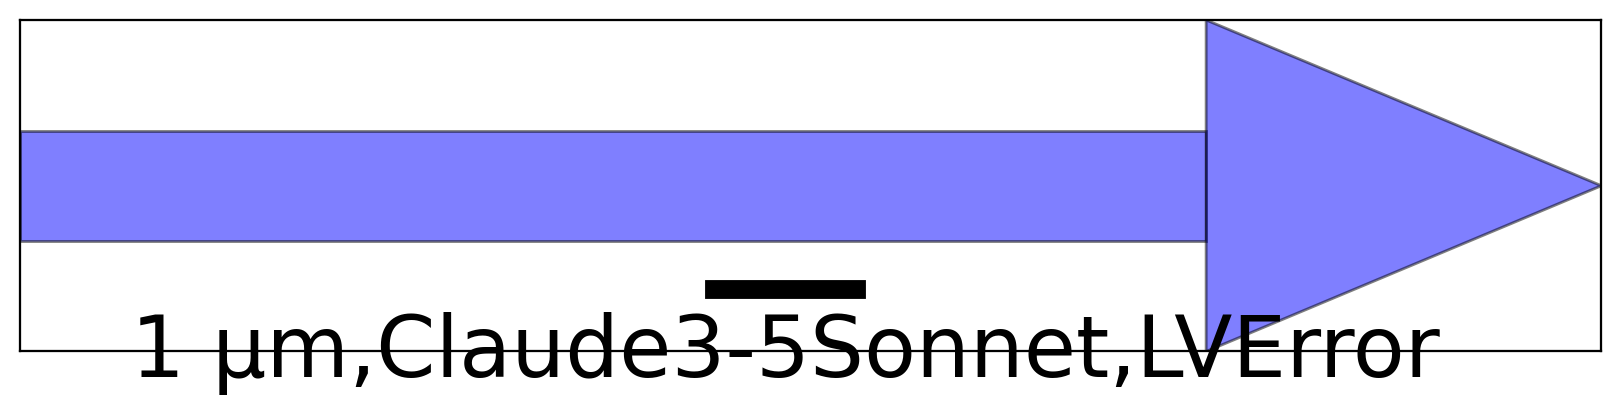
\includegraphics[width=0.13\textwidth]{./run_2/png/claude-3-5-sonnet-20240620_results/Arrow.png} & 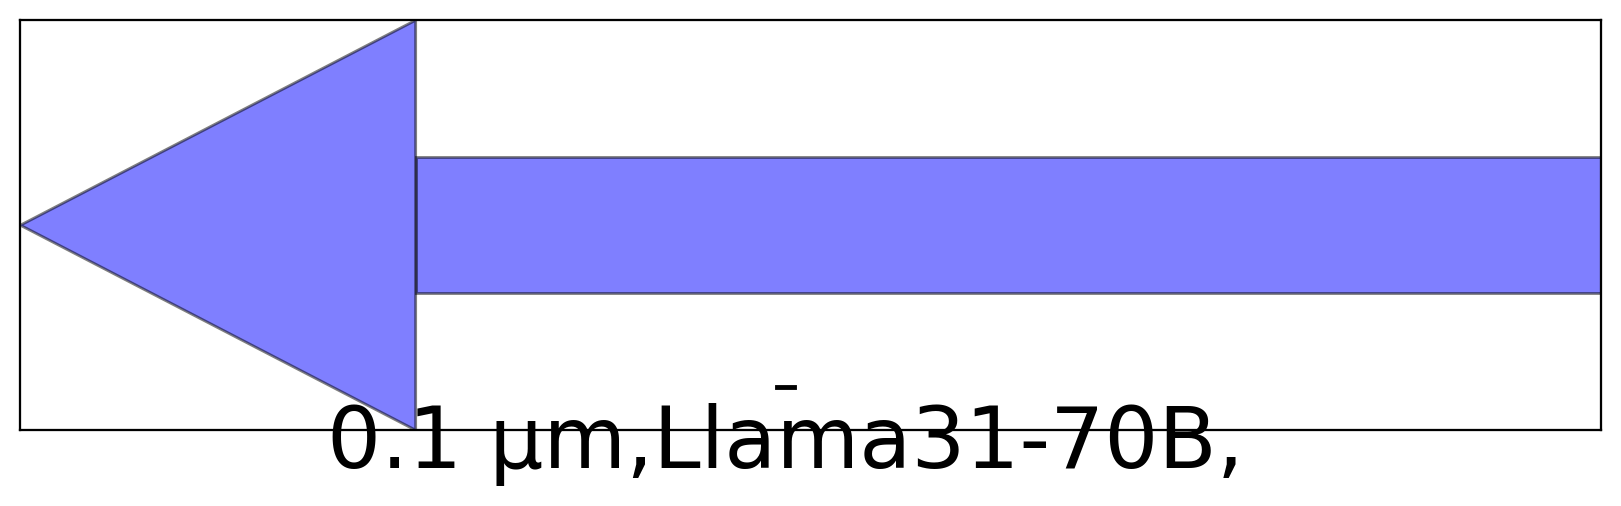
\includegraphics[width=0.13\textwidth]{./run_2/png/watsonx_meta-llama_llama-3-1-70b-instruct_results/Arrow.png} & 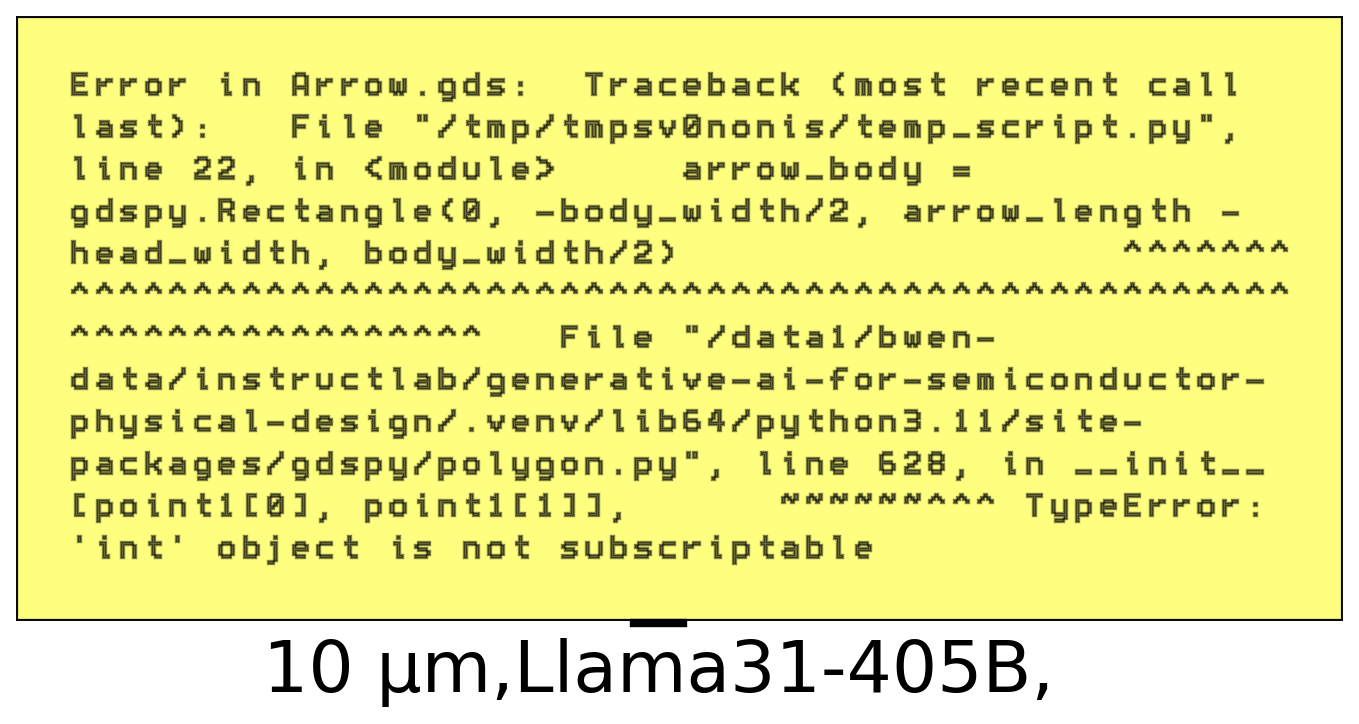
\includegraphics[width=0.13\textwidth]{./run_2/png/watsonx_meta-llama_llama-3-405b-instruct_results/Arrow.png} \\
    \makecell{Single LLM \\ Baseline \\ Run 3} & 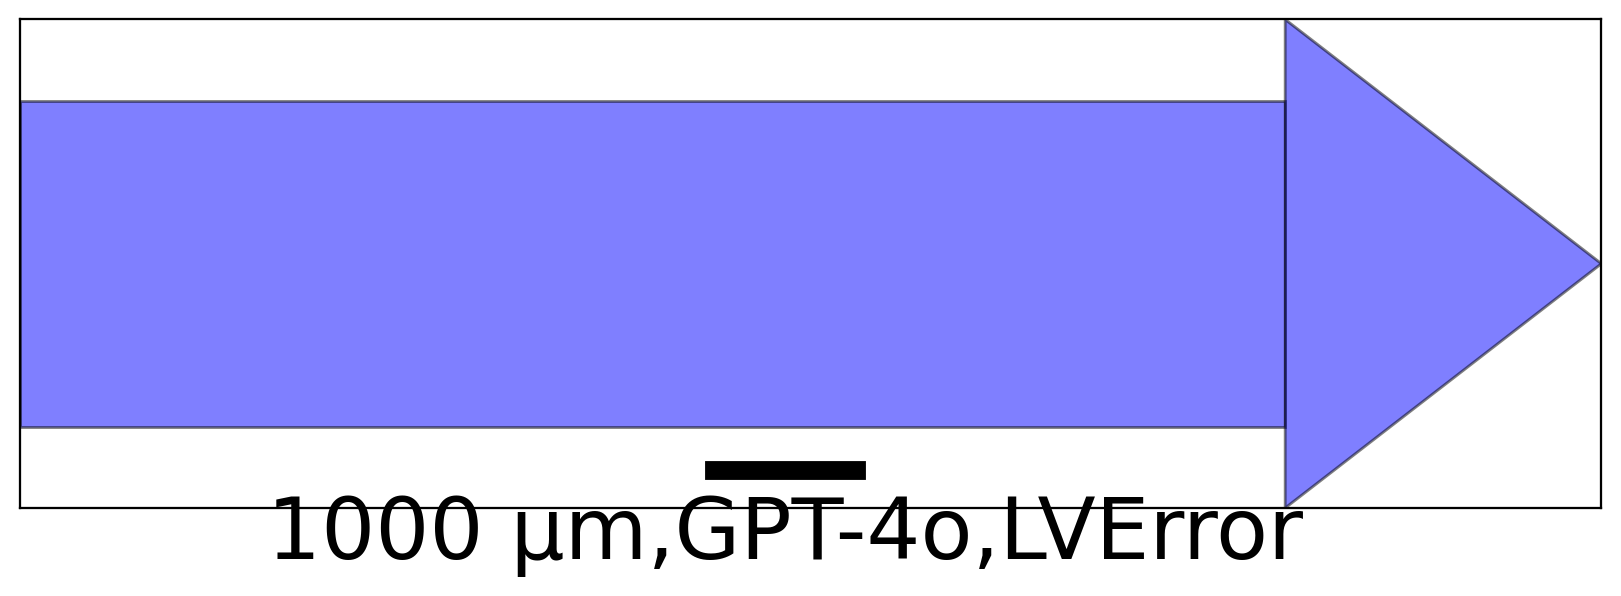
\includegraphics[width=0.13\textwidth]{./run_3/png/gpt-4o_results/Arrow.png} & 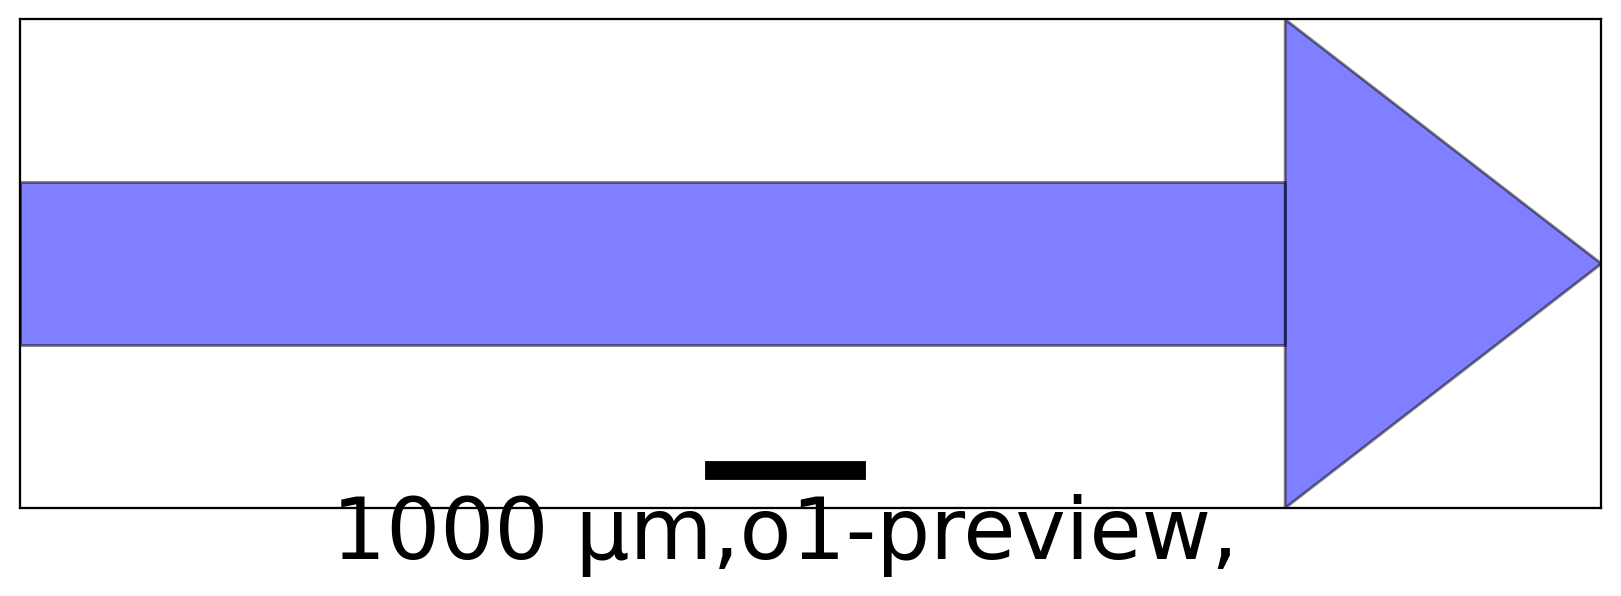
\includegraphics[width=0.13\textwidth]{./run_3/png/o1-preview_results/Arrow.png} & 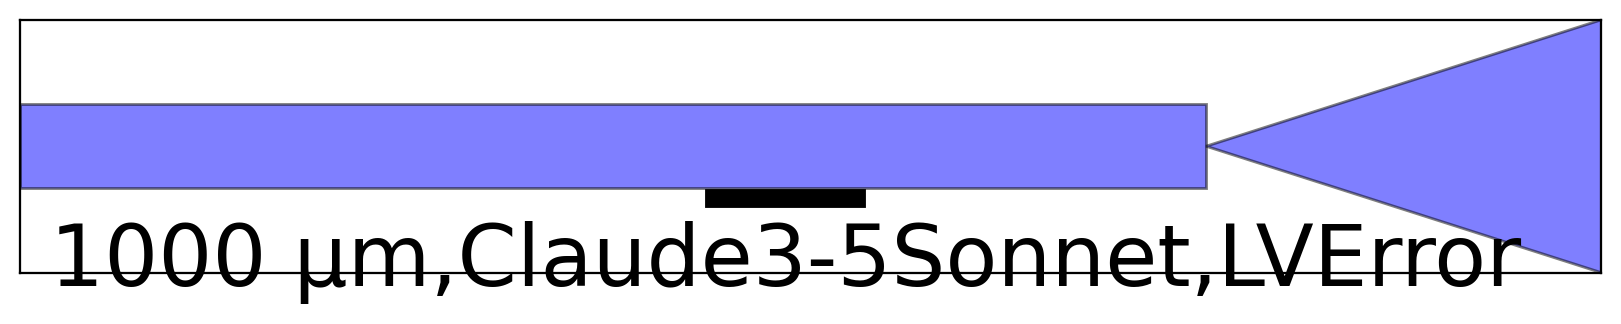
\includegraphics[width=0.13\textwidth]{./run_3/png/claude-3-5-sonnet-20240620_results/Arrow.png} & 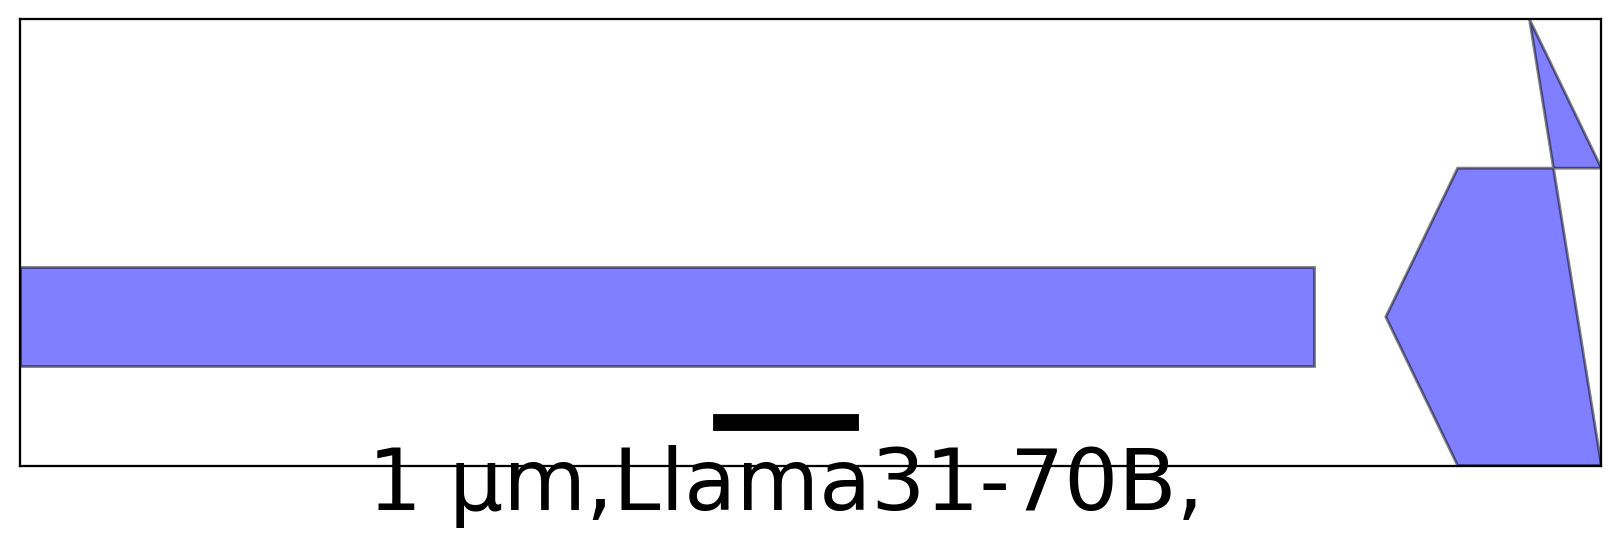
\includegraphics[width=0.13\textwidth]{./run_3/png/watsonx_meta-llama_llama-3-1-70b-instruct_results/Arrow.png} & 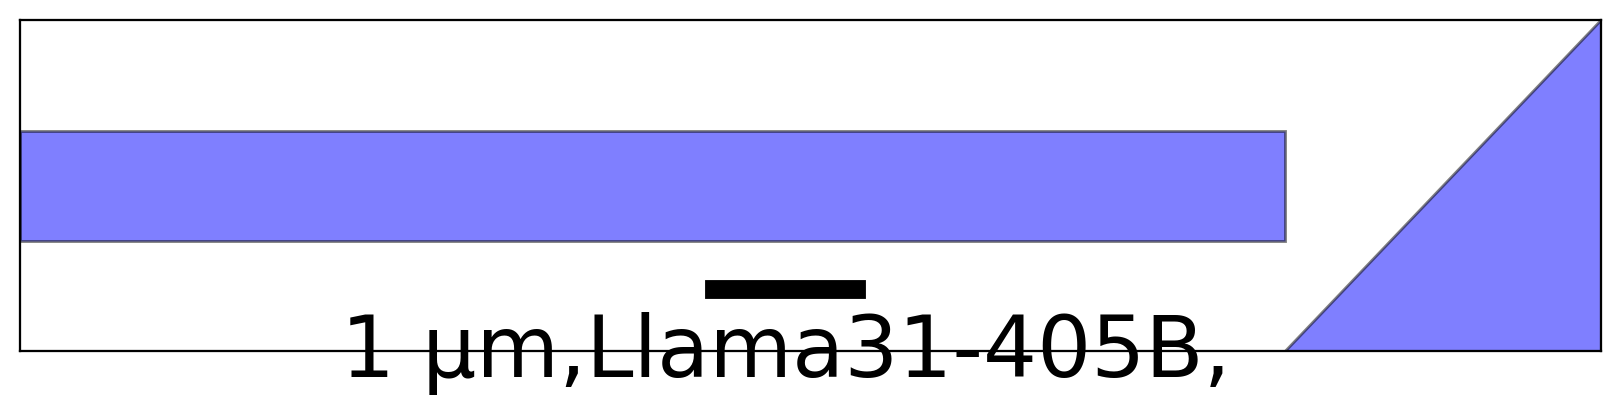
\includegraphics[width=0.13\textwidth]{./run_3/png/watsonx_meta-llama_llama-3-405b-instruct_results/Arrow.png} \\
    \makecell{Single LLM \\ Baseline \\ Run 4} & 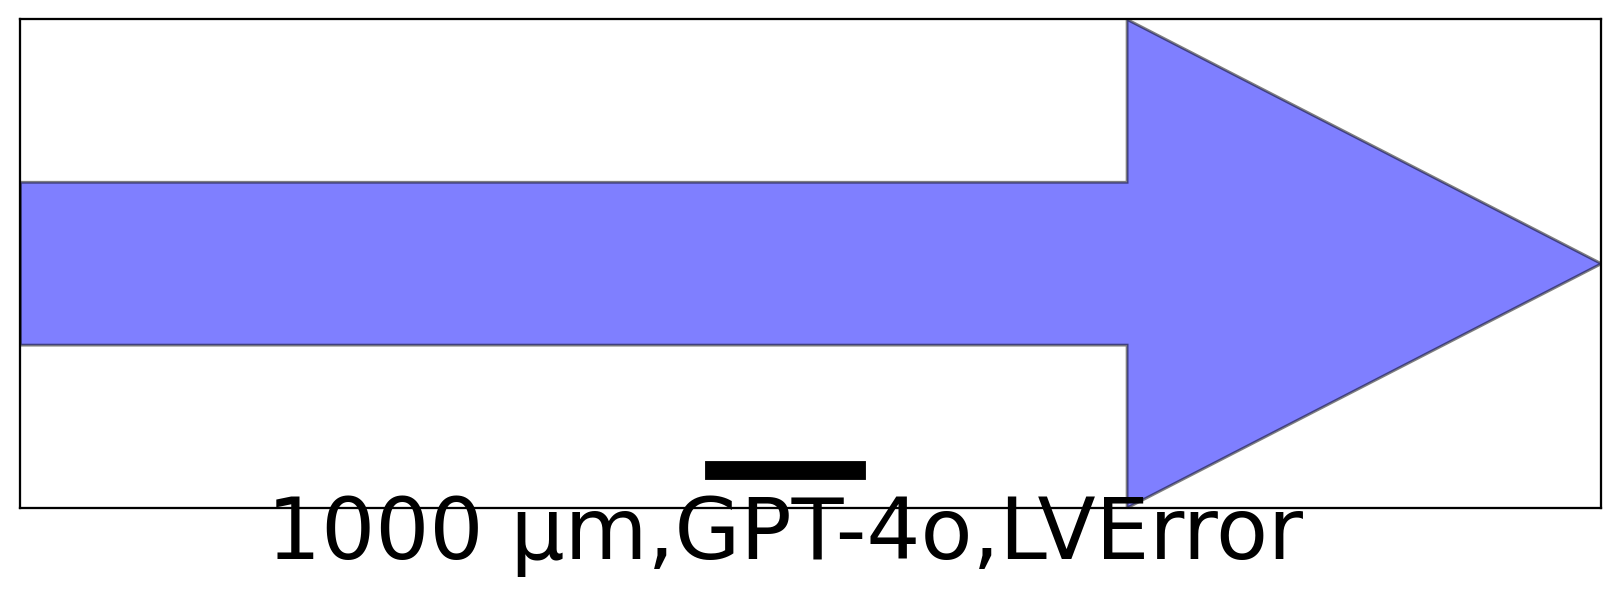
\includegraphics[width=0.13\textwidth]{./run_4/png/gpt-4o_results/Arrow.png} & 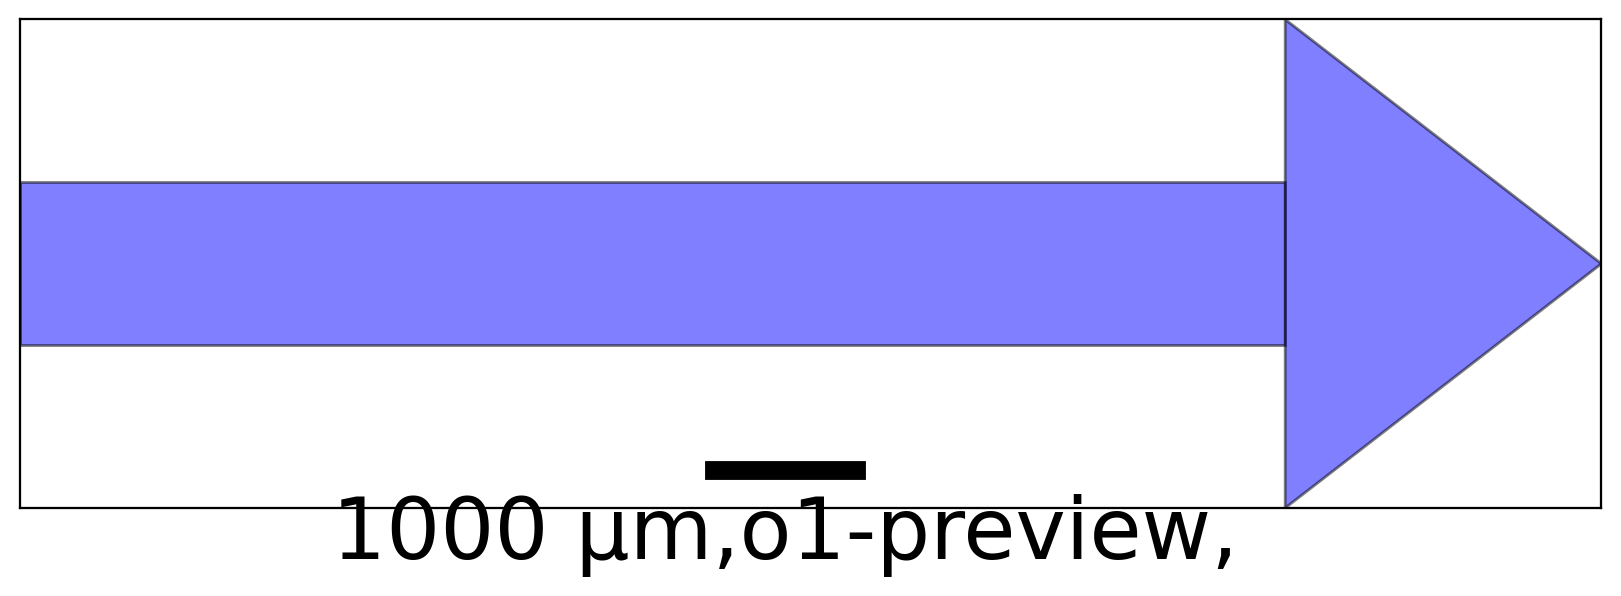
\includegraphics[width=0.13\textwidth]{./run_4/png/o1-preview_results/Arrow.png} & 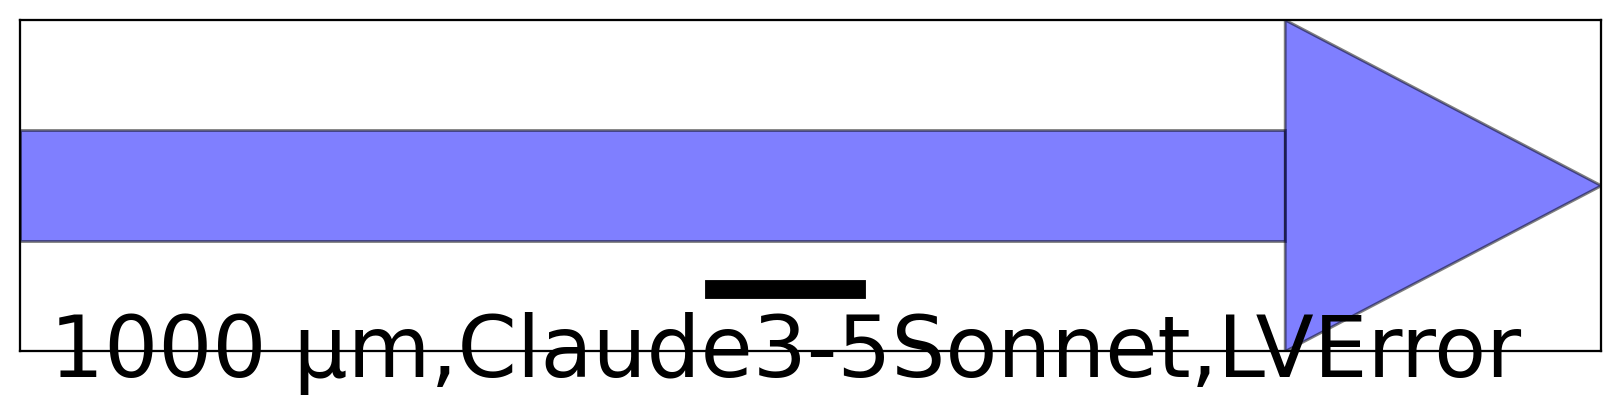
\includegraphics[width=0.13\textwidth]{./run_4/png/claude-3-5-sonnet-20240620_results/Arrow.png} & 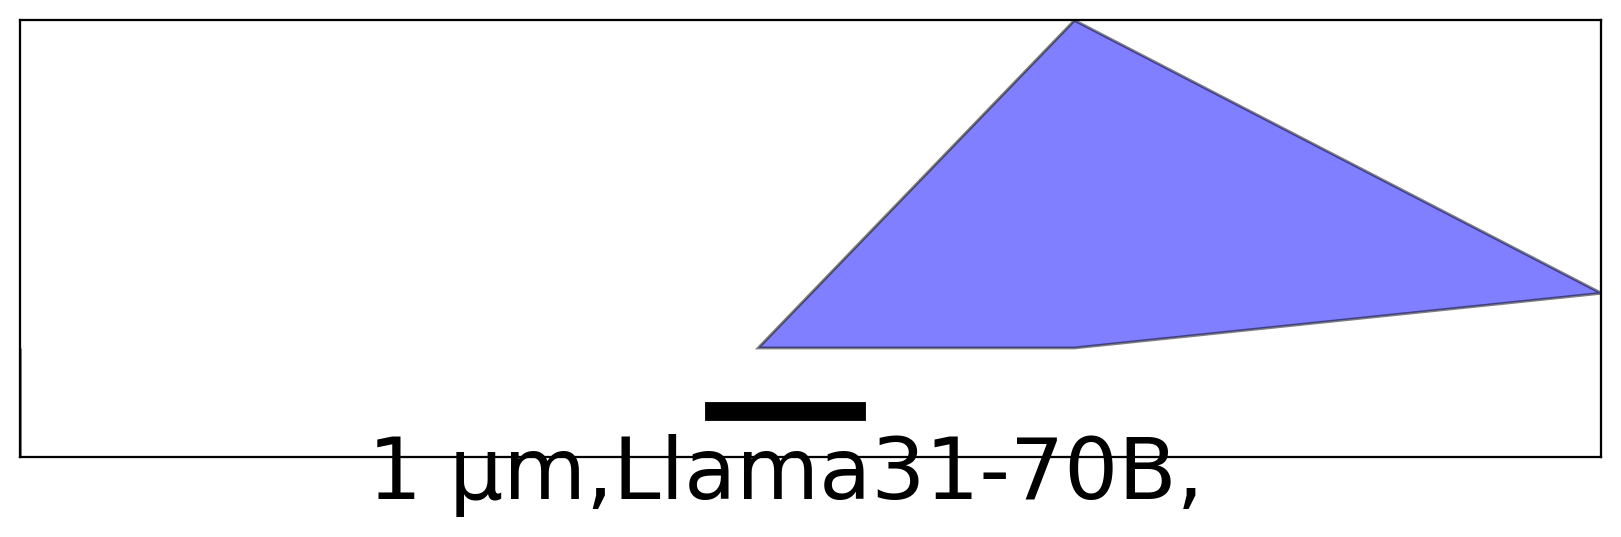
\includegraphics[width=0.13\textwidth]{./run_4/png/watsonx_meta-llama_llama-3-1-70b-instruct_results/Arrow.png} & 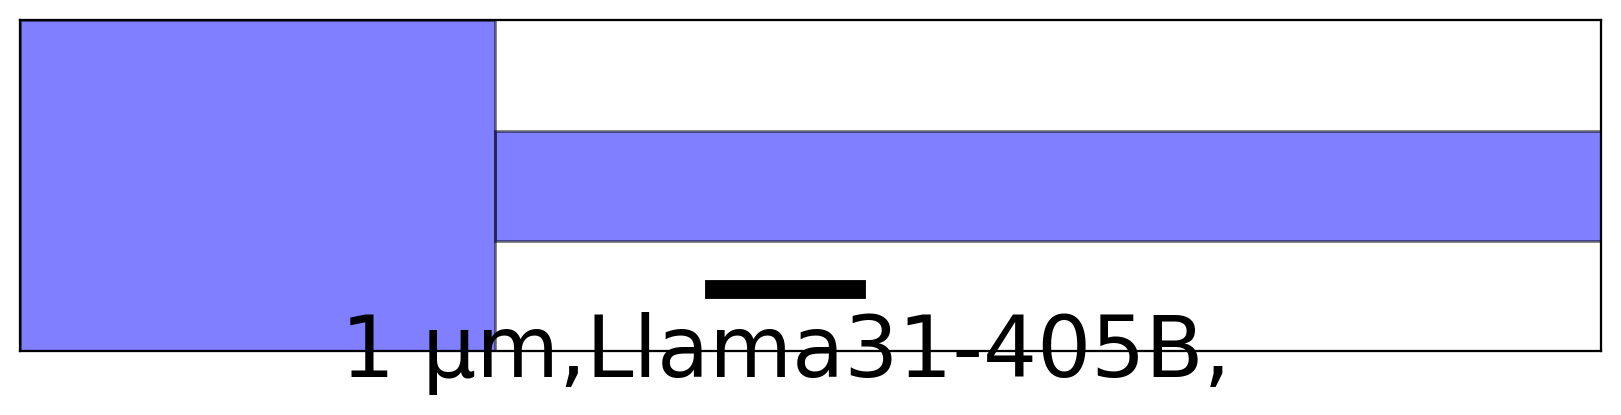
\includegraphics[width=0.13\textwidth]{./run_4/png/watsonx_meta-llama_llama-3-405b-instruct_results/Arrow.png} \\
    \makecell{Single LLM \\ Baseline \\ Run 5} & 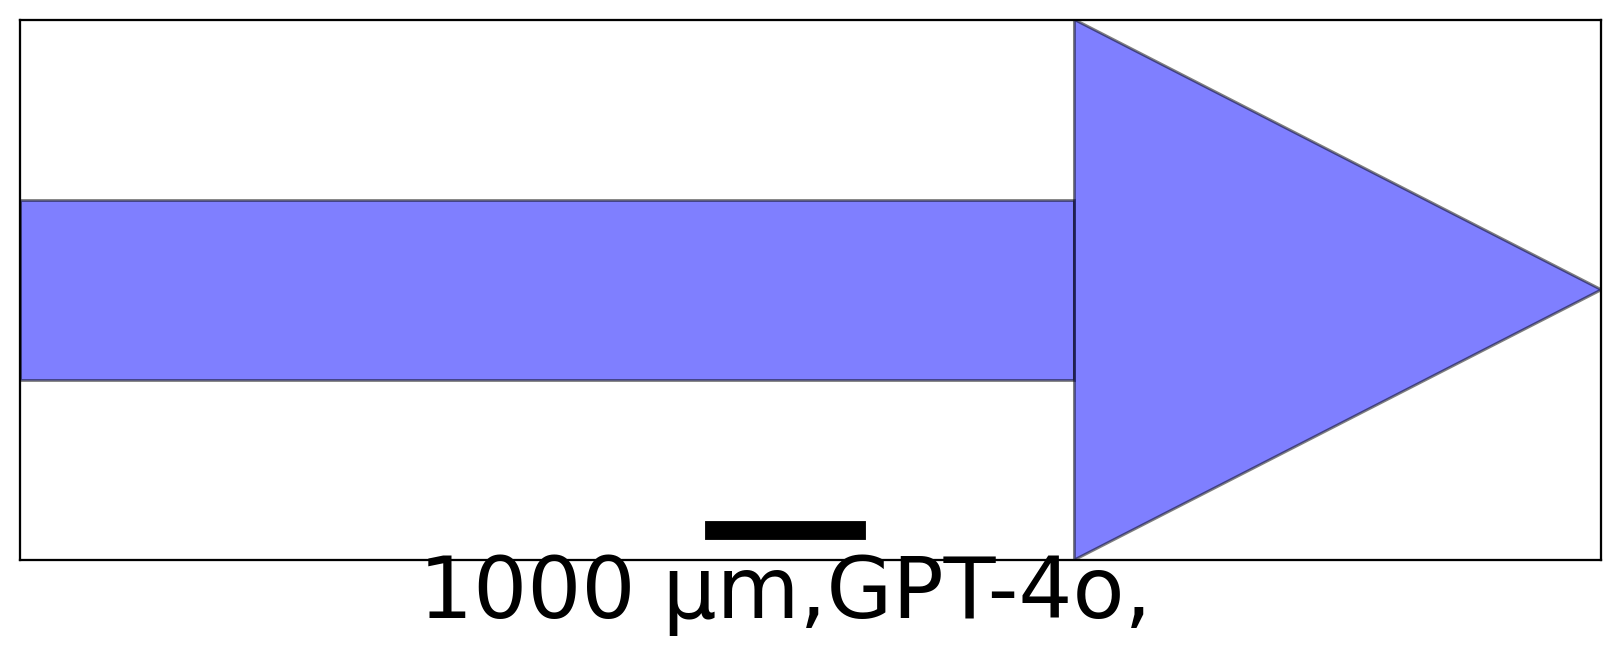
\includegraphics[width=0.13\textwidth]{./run_5/png/gpt-4o_results/Arrow.png} & 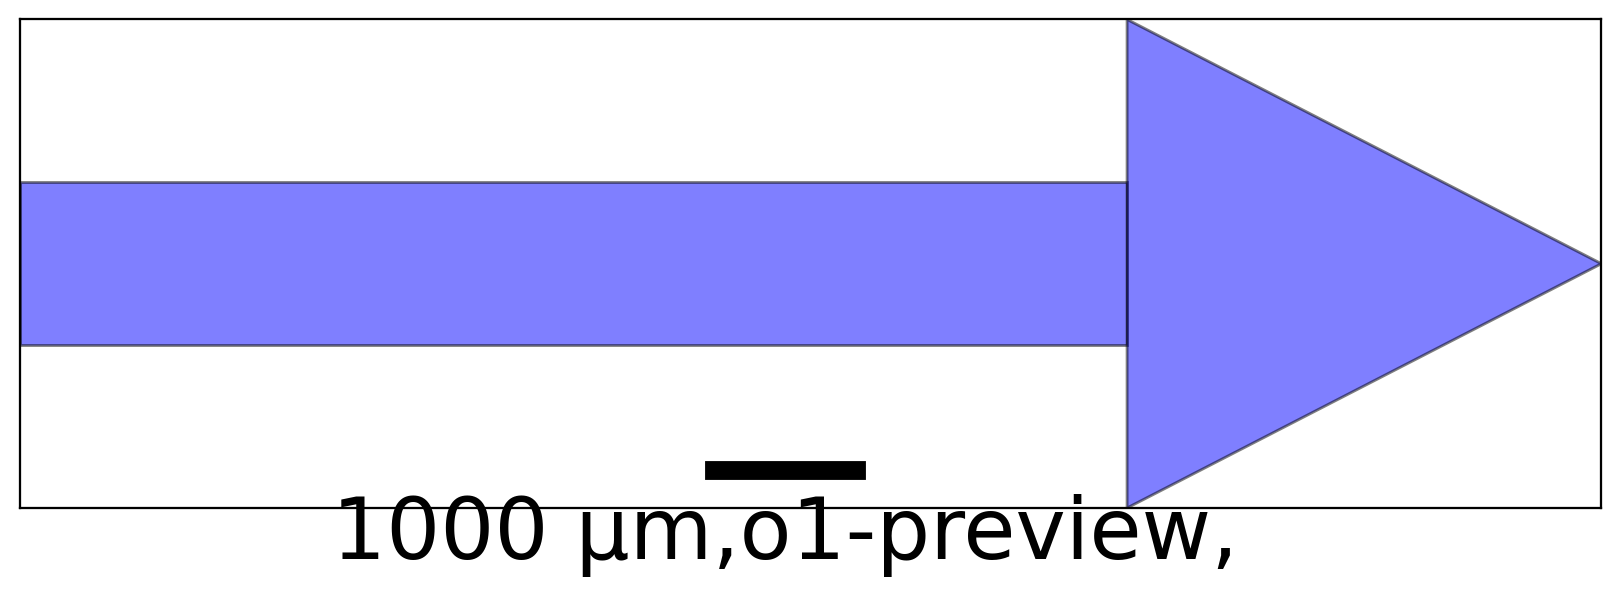
\includegraphics[width=0.13\textwidth]{./run_5/png/o1-preview_results/Arrow.png} & 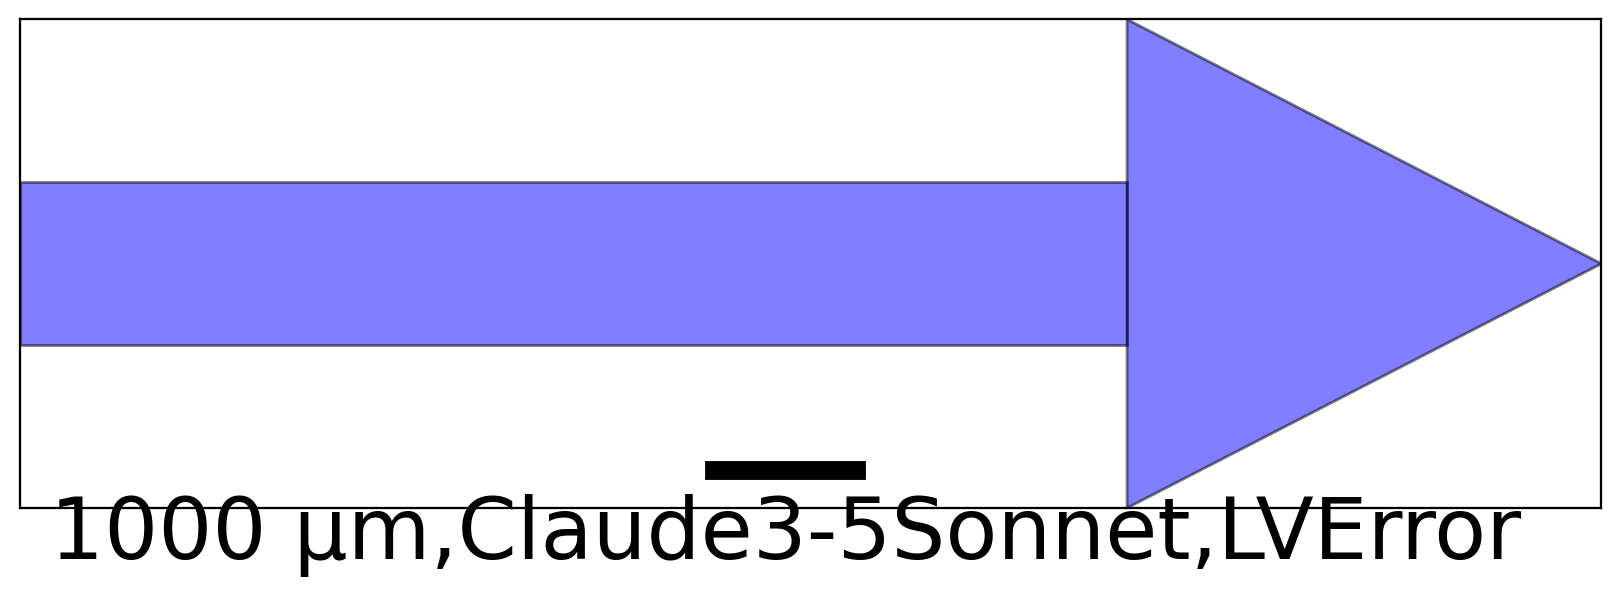
\includegraphics[width=0.13\textwidth]{./run_5/png/claude-3-5-sonnet-20240620_results/Arrow.png} & 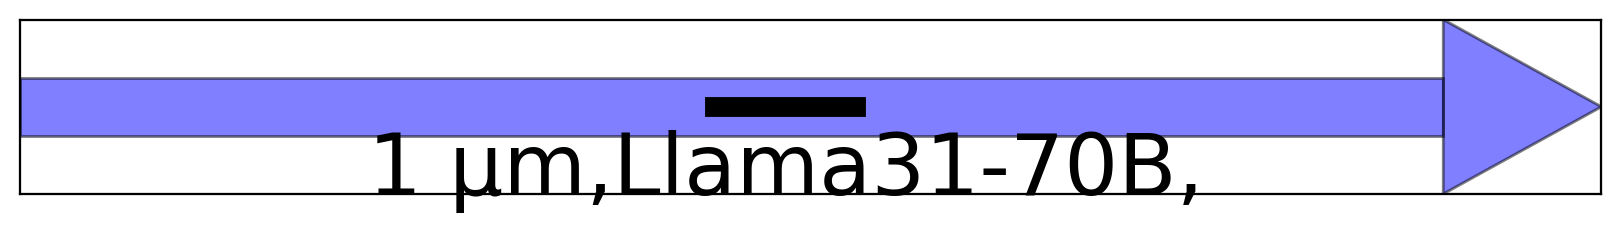
\includegraphics[width=0.13\textwidth]{./run_5/png/watsonx_meta-llama_llama-3-1-70b-instruct_results/Arrow.png} & 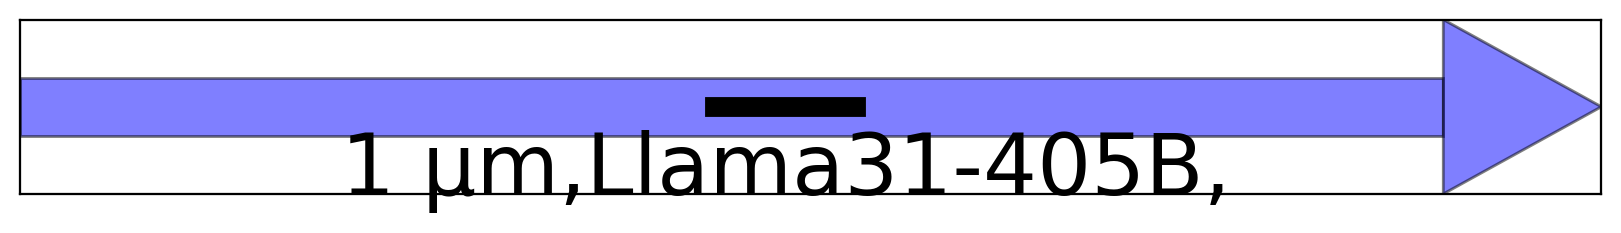
\includegraphics[width=0.13\textwidth]{./run_5/png/watsonx_meta-llama_llama-3-405b-instruct_results/Arrow.png} \\
    \bottomrule
  \end{tabular}
  \caption*{Question: Generate an Arrow pointing to the right with length 10 mm, make the body 1/3 width of the head, start at 0,0.}
\end{table}\begin{table}
  \caption{BasicLayout Task}
  \label{table:basiclayout}
  \centering
  \begin{tabularx}{\textwidth}{@{}XXXXXX@{}}
    \toprule
    \makecell{Ground Truth \\ 
\includegraphics[width=0.13\textwidth]{examples_png/BasicLayout.png}} & GPT-4o & Claude-3.5 & Llama-3-70B & Llama-3-405B & o1-preview \\
    \midrule
    SOLOMON & 
\includegraphics[width=0.13\textwidth]{./pool_all/png/gpt-4o_results/BasicLayout.png} &  & 
\includegraphics[width=0.13\textwidth]{./pool_all/png/claude-3-5-sonnet-20240620_results/BasicLayout.png} & 
\includegraphics[width=0.13\textwidth]{./pool_all/png/watsonx_meta-llama_llama-3-1-70b-instruct_results/BasicLayout.png} & 
\includegraphics[width=0.13\textwidth]{./pool_all/png/watsonx_meta-llama_llama-3-405b-instruct_results/BasicLayout.png} \\
    \makecell{Single LLM \\ Baseline \\ Run 1} & 
\includegraphics[width=0.13\textwidth]{./run_1/png/gpt-4o_results/BasicLayout.png} & 
\includegraphics[width=0.13\textwidth]{./run_1/png/o1-preview_results/BasicLayout.png} & 
\includegraphics[width=0.13\textwidth]{./run_1/png/claude-3-5-sonnet-20240620_results/BasicLayout.png} & 
\includegraphics[width=0.13\textwidth]{./run_1/png/watsonx_meta-llama_llama-3-1-70b-instruct_results/BasicLayout.png} & 
\includegraphics[width=0.13\textwidth]{./run_1/png/watsonx_meta-llama_llama-3-405b-instruct_results/BasicLayout.png} \\
    \makecell{Single LLM \\ Baseline \\ Run 2} & 
\includegraphics[width=0.13\textwidth]{./run_2/png/gpt-4o_results/BasicLayout.png} & 
\includegraphics[width=0.13\textwidth]{./run_2/png/o1-preview_results/BasicLayout.png} & 
\includegraphics[width=0.13\textwidth]{./run_2/png/claude-3-5-sonnet-20240620_results/BasicLayout.png} & 
\includegraphics[width=0.13\textwidth]{./run_2/png/watsonx_meta-llama_llama-3-1-70b-instruct_results/BasicLayout.png} & 
\includegraphics[width=0.13\textwidth]{./run_2/png/watsonx_meta-llama_llama-3-405b-instruct_results/BasicLayout.png} \\
    \makecell{Single LLM \\ Baseline \\ Run 3} & 
\includegraphics[width=0.13\textwidth]{./run_3/png/gpt-4o_results/BasicLayout.png} & 
\includegraphics[width=0.13\textwidth]{./run_3/png/o1-preview_results/BasicLayout.png} & \includegraphics[width=0.13\textwidth]{./run_3/png/claude-3-5-sonnet-20240620_results/BasicLayout.png} & \includegraphics[width=0.13\textwidth]{./run_3/png/watsonx_meta-llama_llama-3-1-70b-instruct_results/BasicLayout.png} & \includegraphics[width=0.13\textwidth]{./run_3/png/watsonx_meta-llama_llama-3-405b-instruct_results/BasicLayout.png} \\
    \makecell{Single LLM \\ Baseline \\ Run 4} & \includegraphics[width=0.13\textwidth]{./run_4/png/gpt-4o_results/BasicLayout.png} & \includegraphics[width=0.13\textwidth]{./run_4/png/o1-preview_results/BasicLayout.png} & \includegraphics[width=0.13\textwidth]{./run_4/png/claude-3-5-sonnet-20240620_results/BasicLayout.png} & \includegraphics[width=0.13\textwidth]{./run_4/png/watsonx_meta-llama_llama-3-1-70b-instruct_results/BasicLayout.png} & \includegraphics[width=0.13\textwidth]{./run_4/png/watsonx_meta-llama_llama-3-405b-instruct_results/BasicLayout.png} \\
    \makecell{Single LLM \\ Baseline \\ Run 5} & \includegraphics[width=0.13\textwidth]{./run_5/png/gpt-4o_results/BasicLayout.png} & \includegraphics[width=0.13\textwidth]{./run_5/png/o1-preview_results/BasicLayout.png} & \includegraphics[width=0.13\textwidth]{./run_5/png/claude-3-5-sonnet-20240620_results/BasicLayout.png} & \includegraphics[width=0.13\textwidth]{./run_5/png/watsonx_meta-llama_llama-3-1-70b-instruct_results/BasicLayout.png} & \includegraphics[width=0.13\textwidth]{./run_5/png/watsonx_meta-llama_llama-3-405b-instruct_results/BasicLayout.png} \\
    \bottomrule
  \end{tabular}
  \caption*{Question: 1. Draw a rectangular active region with dimensions 10 µm x 5 µm.
2. Place a polysilicon gate that crosses the active region vertically at its center, with a width of 1 µm.
3. Add two square contact holes, each 1 µm x 1 µm, positioned 1 µm away from the gate on either side along the active region.}
\end{table}\begin{table}
  \caption{MicrofluidicChip Task}
  \label{table:microfluidicchip}
  \centering
  \begin{tabularx}{\textwidth}{@{}XXXXXX@{}}
    \toprule
    \makecell{Ground Truth \\ \includegraphics[width=0.13\textwidth]{examples_png/MicrofluidicChip.png}} & GPT-4o & Claude-3.5 & Llama-3-70B & Llama-3-405B & o1-preview \\
    \midrule
    SOLOMON & \includegraphics[width=0.13\textwidth]{./pool_all/png/gpt-4o_results/MicrofluidicChip.png} &  & \includegraphics[width=0.13\textwidth]{./pool_all/png/claude-3-5-sonnet-20240620_results/MicrofluidicChip.png} & \includegraphics[width=0.13\textwidth]{./pool_all/png/watsonx_meta-llama_llama-3-1-70b-instruct_results/MicrofluidicChip.png} & \includegraphics[width=0.13\textwidth]{./pool_all/png/watsonx_meta-llama_llama-3-405b-instruct_results/MicrofluidicChip.png} \\
    \makecell{Single LLM \\ Baseline \\ Run 1} & \includegraphics[width=0.13\textwidth]{./run_1/png/gpt-4o_results/MicrofluidicChip.png} & \includegraphics[width=0.13\textwidth]{./run_1/png/o1-preview_results/MicrofluidicChip.png} & \includegraphics[width=0.13\textwidth]{./run_1/png/claude-3-5-sonnet-20240620_results/MicrofluidicChip.png} & \includegraphics[width=0.13\textwidth]{./run_1/png/watsonx_meta-llama_llama-3-1-70b-instruct_results/MicrofluidicChip.png} & \includegraphics[width=0.13\textwidth]{./run_1/png/watsonx_meta-llama_llama-3-405b-instruct_results/MicrofluidicChip.png} \\
    \makecell{Single LLM \\ Baseline \\ Run 2} & \includegraphics[width=0.13\textwidth]{./run_2/png/gpt-4o_results/MicrofluidicChip.png} & \includegraphics[width=0.13\textwidth]{./run_2/png/o1-preview_results/MicrofluidicChip.png} & \includegraphics[width=0.13\textwidth]{./run_2/png/claude-3-5-sonnet-20240620_results/MicrofluidicChip.png} & \includegraphics[width=0.13\textwidth]{./run_2/png/watsonx_meta-llama_llama-3-1-70b-instruct_results/MicrofluidicChip.png} & \includegraphics[width=0.13\textwidth]{./run_2/png/watsonx_meta-llama_llama-3-405b-instruct_results/MicrofluidicChip.png} \\
    \makecell{Single LLM \\ Baseline \\ Run 3} & \includegraphics[width=0.13\textwidth]{./run_3/png/gpt-4o_results/MicrofluidicChip.png} & \includegraphics[width=0.13\textwidth]{./run_3/png/o1-preview_results/MicrofluidicChip.png} & \includegraphics[width=0.13\textwidth]{./run_3/png/claude-3-5-sonnet-20240620_results/MicrofluidicChip.png} & \includegraphics[width=0.13\textwidth]{./run_3/png/watsonx_meta-llama_llama-3-1-70b-instruct_results/MicrofluidicChip.png} & \includegraphics[width=0.13\textwidth]{./run_3/png/watsonx_meta-llama_llama-3-405b-instruct_results/MicrofluidicChip.png} \\
    \makecell{Single LLM \\ Baseline \\ Run 4} & \includegraphics[width=0.13\textwidth]{./run_4/png/gpt-4o_results/MicrofluidicChip.png} & \includegraphics[width=0.13\textwidth]{./run_4/png/o1-preview_results/MicrofluidicChip.png} & \includegraphics[width=0.13\textwidth]{./run_4/png/claude-3-5-sonnet-20240620_results/MicrofluidicChip.png} & \includegraphics[width=0.13\textwidth]{./run_4/png/watsonx_meta-llama_llama-3-1-70b-instruct_results/MicrofluidicChip.png} & \includegraphics[width=0.13\textwidth]{./run_4/png/watsonx_meta-llama_llama-3-405b-instruct_results/MicrofluidicChip.png} \\
    \makecell{Single LLM \\ Baseline \\ Run 5} & \includegraphics[width=0.13\textwidth]{./run_5/png/gpt-4o_results/MicrofluidicChip.png} & \includegraphics[width=0.13\textwidth]{./run_5/png/o1-preview_results/MicrofluidicChip.png} & \includegraphics[width=0.13\textwidth]{./run_5/png/claude-3-5-sonnet-20240620_results/MicrofluidicChip.png} & \includegraphics[width=0.13\textwidth]{./run_5/png/watsonx_meta-llama_llama-3-1-70b-instruct_results/MicrofluidicChip.png} & \includegraphics[width=0.13\textwidth]{./run_5/png/watsonx_meta-llama_llama-3-405b-instruct_results/MicrofluidicChip.png} \\
    \bottomrule
  \end{tabular}
  \caption*{Question: Draw a design of a microfluidic chip. On layer 0, it is the bulk of the chip. It is a 30 * 20 mm rectangle. On layer 2 (via level), draw two circular vias, with 2 mm radius, and 20 mm apart horizontally. On layer 3 (channel level), draw a rectangular shaped channel (width = 1 mm) that connects the two vias at their center.}
\end{table}\begin{table}
  \caption{ViaConnection Task}
  \label{table:viaconnection}
  \centering
  \begin{tabularx}{\textwidth}{@{}XXXXXX@{}}
    \toprule
    \makecell{Ground Truth \\ \includegraphics[width=0.13\textwidth]{examples_png/ViaConnection.png}} & GPT-4o & Claude-3.5 & Llama-3-70B & Llama-3-405B & o1-preview \\
    \midrule
    SOLOMON & \includegraphics[width=0.13\textwidth]{./pool_all/png/gpt-4o_results/ViaConnection.png} &  & \includegraphics[width=0.13\textwidth]{./pool_all/png/claude-3-5-sonnet-20240620_results/ViaConnection.png} & \includegraphics[width=0.13\textwidth]{./pool_all/png/watsonx_meta-llama_llama-3-1-70b-instruct_results/ViaConnection.png} & \includegraphics[width=0.13\textwidth]{./pool_all/png/watsonx_meta-llama_llama-3-405b-instruct_results/ViaConnection.png} \\
    \makecell{Single LLM \\ Baseline \\ Run 1} & \includegraphics[width=0.13\textwidth]{./run_1/png/gpt-4o_results/ViaConnection.png} & \includegraphics[width=0.13\textwidth]{./run_1/png/o1-preview_results/ViaConnection.png} & \includegraphics[width=0.13\textwidth]{./run_1/png/claude-3-5-sonnet-20240620_results/ViaConnection.png} & \includegraphics[width=0.13\textwidth]{./run_1/png/watsonx_meta-llama_llama-3-1-70b-instruct_results/ViaConnection.png} & \includegraphics[width=0.13\textwidth]{./run_1/png/watsonx_meta-llama_llama-3-405b-instruct_results/ViaConnection.png} \\
    \makecell{Single LLM \\ Baseline \\ Run 2} & \includegraphics[width=0.13\textwidth]{./run_2/png/gpt-4o_results/ViaConnection.png} & \includegraphics[width=0.13\textwidth]{./run_2/png/o1-preview_results/ViaConnection.png} & \includegraphics[width=0.13\textwidth]{./run_2/png/claude-3-5-sonnet-20240620_results/ViaConnection.png} & \includegraphics[width=0.13\textwidth]{./run_2/png/watsonx_meta-llama_llama-3-1-70b-instruct_results/ViaConnection.png} & \includegraphics[width=0.13\textwidth]{./run_2/png/watsonx_meta-llama_llama-3-405b-instruct_results/ViaConnection.png} \\
    \makecell{Single LLM \\ Baseline \\ Run 3} & \includegraphics[width=0.13\textwidth]{./run_3/png/gpt-4o_results/ViaConnection.png} & \includegraphics[width=0.13\textwidth]{./run_3/png/o1-preview_results/ViaConnection.png} & \includegraphics[width=0.13\textwidth]{./run_3/png/claude-3-5-sonnet-20240620_results/ViaConnection.png} & \includegraphics[width=0.13\textwidth]{./run_3/png/watsonx_meta-llama_llama-3-1-70b-instruct_results/ViaConnection.png} & \includegraphics[width=0.13\textwidth]{./run_3/png/watsonx_meta-llama_llama-3-405b-instruct_results/ViaConnection.png} \\
    \makecell{Single LLM \\ Baseline \\ Run 4} & \includegraphics[width=0.13\textwidth]{./run_4/png/gpt-4o_results/ViaConnection.png} & \includegraphics[width=0.13\textwidth]{./run_4/png/o1-preview_results/ViaConnection.png} & \includegraphics[width=0.13\textwidth]{./run_4/png/claude-3-5-sonnet-20240620_results/ViaConnection.png} & \includegraphics[width=0.13\textwidth]{./run_4/png/watsonx_meta-llama_llama-3-1-70b-instruct_results/ViaConnection.png} & \includegraphics[width=0.13\textwidth]{./run_4/png/watsonx_meta-llama_llama-3-405b-instruct_results/ViaConnection.png} \\
    \makecell{Single LLM \\ Baseline \\ Run 5} & \includegraphics[width=0.13\textwidth]{./run_5/png/gpt-4o_results/ViaConnection.png} & \includegraphics[width=0.13\textwidth]{./run_5/png/o1-preview_results/ViaConnection.png} & \includegraphics[width=0.13\textwidth]{./run_5/png/claude-3-5-sonnet-20240620_results/ViaConnection.png} & \includegraphics[width=0.13\textwidth]{./run_5/png/watsonx_meta-llama_llama-3-1-70b-instruct_results/ViaConnection.png} & \includegraphics[width=0.13\textwidth]{./run_5/png/watsonx_meta-llama_llama-3-405b-instruct_results/ViaConnection.png} \\
    \bottomrule
  \end{tabular}
  \caption*{Question: Create a design with three layers: via layer (yellow), metal layer (blue), and pad layer (red). The via radius is 10 units, pad radius is 30 units, and metal connection width is 40 units with a total length of 600 units. Position the first via at (50, 150) and the second via at (550, 150). Ensure the metal connection fully covers the vias and leaves a margin of 10 units between the edge of the metal and the pads. Leave a space of 50 units between the vias and the edges of the metal connection.}
\end{table}\begin{table}
  \caption{DLDChip Task}
  \label{table:dldchip}
  \centering
  \begin{tabularx}{\textwidth}{@{}XXXXXX@{}}
    \toprule
    \makecell{Ground Truth \\ \includegraphics[width=0.13\textwidth]{examples_png/DLDChip.png}} & GPT-4o & Claude-3.5 & Llama-3-70B & Llama-3-405B & o1-preview \\
    \midrule
    SOLOMON & \includegraphics[width=0.13\textwidth]{./pool_all/png/gpt-4o_results/DLDChip.png} &  & \includegraphics[width=0.13\textwidth]{./pool_all/png/claude-3-5-sonnet-20240620_results/DLDChip.png} & \includegraphics[width=0.13\textwidth]{./pool_all/png/watsonx_meta-llama_llama-3-1-70b-instruct_results/DLDChip.png} & \includegraphics[width=0.13\textwidth]{./pool_all/png/watsonx_meta-llama_llama-3-405b-instruct_results/DLDChip.png} \\
    \makecell{Single LLM \\ Baseline \\ Run 1} & \includegraphics[width=0.13\textwidth]{./run_1/png/gpt-4o_results/DLDChip.png} & \includegraphics[width=0.13\textwidth]{./run_1/png/o1-preview_results/DLDChip.png} & \includegraphics[width=0.13\textwidth]{./run_1/png/claude-3-5-sonnet-20240620_results/DLDChip.png} & \includegraphics[width=0.13\textwidth]{./run_1/png/watsonx_meta-llama_llama-3-1-70b-instruct_results/DLDChip.png} & \includegraphics[width=0.13\textwidth]{./run_1/png/watsonx_meta-llama_llama-3-405b-instruct_results/DLDChip.png} \\
    \makecell{Single LLM \\ Baseline \\ Run 2} & \includegraphics[width=0.13\textwidth]{./run_2/png/gpt-4o_results/DLDChip.png} & \includegraphics[width=0.13\textwidth]{./run_2/png/o1-preview_results/DLDChip.png} & \includegraphics[width=0.13\textwidth]{./run_2/png/claude-3-5-sonnet-20240620_results/DLDChip.png} & \includegraphics[width=0.13\textwidth]{./run_2/png/watsonx_meta-llama_llama-3-1-70b-instruct_results/DLDChip.png} & \includegraphics[width=0.13\textwidth]{./run_2/png/watsonx_meta-llama_llama-3-405b-instruct_results/DLDChip.png} \\
    \makecell{Single LLM \\ Baseline \\ Run 3} & \includegraphics[width=0.13\textwidth]{./run_3/png/gpt-4o_results/DLDChip.png} & \includegraphics[width=0.13\textwidth]{./run_3/png/o1-preview_results/DLDChip.png} & \includegraphics[width=0.13\textwidth]{./run_3/png/claude-3-5-sonnet-20240620_results/DLDChip.png} & \includegraphics[width=0.13\textwidth]{./run_3/png/watsonx_meta-llama_llama-3-1-70b-instruct_results/DLDChip.png} & \includegraphics[width=0.13\textwidth]{./run_3/png/watsonx_meta-llama_llama-3-405b-instruct_results/DLDChip.png} \\
    \makecell{Single LLM \\ Baseline \\ Run 4} & \includegraphics[width=0.13\textwidth]{./run_4/png/gpt-4o_results/DLDChip.png} & \includegraphics[width=0.13\textwidth]{./run_4/png/o1-preview_results/DLDChip.png} & \includegraphics[width=0.13\textwidth]{./run_4/png/claude-3-5-sonnet-20240620_results/DLDChip.png} & \includegraphics[width=0.13\textwidth]{./run_4/png/watsonx_meta-llama_llama-3-1-70b-instruct_results/DLDChip.png} & \includegraphics[width=0.13\textwidth]{./run_4/png/watsonx_meta-llama_llama-3-405b-instruct_results/DLDChip.png} \\
    \makecell{Single LLM \\ Baseline \\ Run 5} & \includegraphics[width=0.13\textwidth]{./run_5/png/gpt-4o_results/DLDChip.png} & \includegraphics[width=0.13\textwidth]{./run_5/png/o1-preview_results/DLDChip.png} & \includegraphics[width=0.13\textwidth]{./run_5/png/claude-3-5-sonnet-20240620_results/DLDChip.png} & \includegraphics[width=0.13\textwidth]{./run_5/png/watsonx_meta-llama_llama-3-1-70b-instruct_results/DLDChip.png} & \includegraphics[width=0.13\textwidth]{./run_5/png/watsonx_meta-llama_llama-3-405b-instruct_results/DLDChip.png} \\
    \bottomrule
  \end{tabular}
  \caption*{Question: Draw a deterministic lateral displacement chip - include channel that can hold the array has gap size = 225 nm, circular pillar size = 400 nm, width = 30 pillars, row shift fraction = 0.1, add an inlet and outlet 40 µm diameter before and after the channel, use a 20*50 µm bus to connect the inlet and outlet to the channel.}
\end{table}

This comprehensive presentation of tasks, prompts, ground truths, and LLM outputs provides a clear view of the performance and capabilities of different models in generating GDSII layouts. It allows for easy comparison between the expected results and the actual outputs from various LLMs and the SOLOMON system.

\subsection{Errors in Baseline Experiment}
\label{appendix:baseline_errors}

\subsubsection{Scaling Errors}
\label{appendix:scaling_errors}

The default unit in the gdspy library is micrometers. We requested basic shapes to be drawn in millimeters to test whether LLMs could correctly handle this unit conversion. All LLMs struggled to various degrees:

(a) Some LLMs failed to pay attention to the requested unit (millimeters) and did not perform the necessary scaling.

(b) In some cases, LLMs paid attention to the requested unit but made incorrect assumptions about gdspy's default unit. We observed biased hallucinations: Llama models tended to assume millimeters, Claude models sometimes defaulted to nanometers, while GPT-4o occasionally interpreted the default unit as meters.

(c) As mentioned in the main text, Llama-3 models were especially vulnerable to this issue. They sometimes assumed the user had made a mistake by requesting millimeters, and proceeded to draw in micrometers instead, justifying this choice with comments like "not mm, as the GDSII format is in micrometers". This type of "arrogant" behavior and misalignment with human instructions on simple tasks could be harmful for deploying LLMs as fully autonomous AI agents. A recent Nature paper \cite{ZhouNature2024} has also discussed similar observations.

\subsubsection{Shape Errors}
\label{appendix:shape_errors}

Incorrect shapes often resulted from LLMs making basic arithmetic errors. For instance, in the "Hexagon" task, Llama-3.1-405B once used an internal angle of 120 degrees, producing a triangle instead of a hexagon. However, in other runs, it correctly calculated the angle based on the number of edges. Many of these errors can be mitigated through Chain-of-Thought (CoT) prompting, which encourages the model to do calculations step-by-step.

\subsubsection{Runtime Errors}
\label{appendix:runtime_errors}

This section provides a detailed breakdown of the errors encountered during the baseline experiment for each LLM. The most frequent error across all models was \textit{AttributeError: module 'gdspy' has no attribute 'LayoutViewer'}, occurring 26 times (59.09\%) with GPT-4o and 33 times (61.11\%) with Claude-3.5-Sonnet. This error was less common in other models, appearing only once each for Llama-3.1-70B and o1-preview, and not at all for Llama-3.1-405B.

The prevalence of this error indicates that GPT-4o and Claude-3.5-Sonnet attempted to provide GUI output, which was unavailable in the runtime environment. However, this issue stems from a lack of specification about the runtime environment in the prompt, rather than being entirely the LLMs' fault.

To ensure a fair comparison, we re-ran all generated code with `LayoutViewer` lines commented out. The analysis presented in Figure \ref{fig:baseline-llm-performance} and the following breakdown reflect these adjusted results.

Other common errors included hallucinations of nonexistent `gdspy` functions or methods, resulting in various `AttributeErrors` (e.g., `'CrossSection'`, `'Circular'`, `'Ellipse'`) and `TypeErrors`. Some errors were due to spelling mistakes, such as misspelling \textit{gdspy.Text} as \textit{gdspy.text}.

The subsequent analysis presents a detailed error breakdown for each LLM, ranked by ascending number of errors.

\paragraph{o1-preview}
Total errors: 12

The main errors for o1-preview included:
\begin{itemize}
    \item TypeError: GdsLibrary.write\_gds() got an unexpected keyword argument 'unit' (16.67\%)
    \item SyntaxError: invalid syntax (16.67\%)
    \item Various TypeErrors and AttributeErrors related to unexpected keyword arguments or missing attributes (66.66\%)
\end{itemize}

\paragraph{GPT-4o}
Total errors: 18

The most common errors for GPT-4o were:
\begin{itemize}
    \item TypeError related to unexpected keyword arguments (27.78\%)
    \item SyntaxError: invalid syntax (16.67\%)
    \item TypeError: 'float' object cannot be interpreted as an integer (11.11\%)
\end{itemize}

Other errors included various AttributeErrors, IndexErrors, and ValueErrors, each occurring once or twice.

\paragraph{Claude-3-5-sonnet}
Total errors: 21

The most frequent error for Claude-3-5-sonnet was:
\begin{itemize}
    \item TypeError: Text.\_\_init\_\_() got an unexpected keyword argument 'anchor' (38.10\%)
\end{itemize}

Other errors included:
\begin{itemize}
    \item TypeError: Path.\_\_init\_\_() got an unexpected keyword argument 'layer' (9.52\%)
    \item Various TypeErrors, ValueErrors, and AttributeErrors, each occurring once (52.38\%)
\end{itemize}

\paragraph{Llama-3-405b}
Total errors: 36

The most frequent errors for Llama-3-405b were:
\begin{itemize}
    \item TypeError: 'int' object is not subscriptable (8.33\%)
    \item SyntaxError: invalid syntax (8.33\%)
    \item Various TypeErrors related to unexpected keyword arguments or multiple values for arguments (16.68\%)
\end{itemize}

This model also encountered several ValueErrors and AttributeErrors.

\paragraph{Llama-3-70b}
Total errors: 68

The most prevalent error for Llama-3-70b was:
\begin{itemize}
    \item AttributeError: module 'gdspy' has no attribute 'Library'. Did you mean: 'library'? (36.76\%)
\end{itemize}

Other common errors included:
\begin{itemize}
    \item TypeError: GdsLibrary.write\_gds() got an unexpected keyword argument 'unit' (7.35\%)
    \item SyntaxError related to assignment (5.88\%)
    \item Various TypeErrors and AttributeErrors related to unexpected keyword arguments or missing attributes (25.00\%)
\end{itemize}

These error patterns suggest that all models struggled with correctly using the gdspy library, often attempting to use non-existent attributes or passing incorrect arguments to functions. Syntax errors were also common across models, indicating issues with code structure and Python syntax.

\subsubsection{Inefficient Code Example}
\label{appendix:inefficient_code}

In the DLDChip task, which involves creating a dense array of identical shapes, the Llama-3.1-405B model generated code that created a large number of objects and performed numerous boolean operations. This led to high memory usage and extended execution time, requiring the code to be terminated after approximately 15 minutes of runtime.

\subsubsection{Ambiguous Instructions}
\label{appendix:ambiguous_instructions}

In some cases, we observed that the LLM results mainly fell into two categories. After inspecting the prompts, we found that the instructions could be interpreted in two ways. In these cases, we counted both types of results as correct. However, when implementing a copilot, the agent should ask for clarification if the instructions are ambiguous.

\subsection{Via Connection Test Cases}
\label{appendix:via_connection}

Figure \ref{fig:sketch} shows the sketch used in all via connection test cases discussed in Section \ref{sec:multimodal_inputs}.

\begin{figure}[h]
\centering
\includegraphics[width=0.5\linewidth]{sketch.png}
\caption{Sketch used for via connection test cases}
\label{fig:sketch}
\end{figure}

\subsubsection{Prompts for Via Connection Tests}
\label{appendix:via_prompts}

\textbf{Test 1:} "I have a sketch idea that i want to draw in GDSII, generate the python code for this design. each color represents an individual layer. We want to use a metal to connect two vias and put a pad on top of each via"

\textbf{Test 2:} "I have a sketch idea that i want to draw in GDSII, generate the python code for this design. each color represents an individual layer. We want to have two vias near each end on a piece of metal. And a pad on top of the metal."

\textbf{Test 3:} "I have a sketch idea that i want to draw in GDSII, generate the python code for this design. each color represents an individual layer. we want use to connect two vias using a piece of metal and put a circular padding on top of each via"

Figure \ref{fig:test3_chat} illustrates the iterative prompting process for Test 3, as discussed in Section \ref{sec:multimodal_inputs}.

\begin{figure}[!h]
\centering
\includegraphics[width=0.5\linewidth]{Styles/Test3.png}
\caption{Test 3 - Iterations to guide the model to generate desired output}
\label{fig:test3_chat}
\end{figure}

\textbf{Test 4 (Generated by LLM based on the final output in Test 3):}\\
"Layers and Colors:
The design consists of three layers: via layer (yellow), metal layer (blue), and pad layer (red).\\
Dimensions:
Via: The radius of each via is 10 units.
Pad: The radius of each pad is 30 units.
Metal Connection: The width of the metal connection is 40 units, and the total length is 600 units.\\
Positions:
The first via is positioned at coordinates (50, 150).
The second via is positioned at coordinates (550, 150).\\
Connections and Coverage:
The metal connection should fully cover the vias, extending slightly beyond their edges.
Ensure the metal connection is slightly wider than the via diameter to provide full coverage.\\
Spacing and Margins:
Leave a margin of 10 units between the edge of the metal and the pads.
Ensure there is a space of 50 units between the vias and the edges of the metal connection.\\
Additional Requirements:
The metal connection should be shorter than the total length to fit beneath the covering area of the pads, leaving some space at the edges.
By providing detailed information like this, you can ensure that the design is accurately reproduced. If you have any specific design rules or preferences, make sure to include those as well."

\textbf{Test 5:} "I have sketched a design for 3d packaging, where we have a metal connecting two TSVs , please generate the python code to draw a GDSII for this design."

\textbf{Test 6:} "I have sketched a design for 3d packaging, where we have a metal connecting two TSVs , please generate the python code to draw a GDSII based on the sketch. each color represents an individual layer. The metal connection should fully cover the vias, extending slightly beyond their edges. Ensure the metal connection is slightly wider than the via diameter to provide full coverage."

\end{document}
